\setlength{\parindent}{0em} 

%**********************************************************************************
% Kapitel Best-Practice-Ansätze
%**********************************************************************************
\chapter{Best-Practice-Ansätze}
\label{cha:Auswertung}
In diesem Kapitel wird versucht, die in Kapitel \ref{kap_anforderungsmatrix_abgleitete_maßnahmen} abgeleiteten technischen Maßnahmen in Bereiche zu Gruppieren. Auf Basis dieser Gruppen werden die einzelnen Maßnahmen beschrieben und Best-Practice-Ansätze definiert um eine umfassende und effiziente Adressierung der Maßnahmen zu ermöglichen. Die Gruppierung hat sich im Zuge der Ausarbeitung als sinnvoll ergeben, da unterschiedliche Maßnahmen ineinander greifen und voneinander profitieren.  
\bigbreak
Unter einem Best-Practice-Ansatz kann eine bestmögliche, bereits erprobte Methode oder Maßnahme zur Umsetzung einer Problemstellung verstanden werden. Ein Best-Practice-Ansatz stellt allerdings im allgemeinen Sprachgebrauch nur eine unverbindliche Empfehlung dar und unterscheidet sich somit von einem etablierten Standard. Die Empfehlung kann aufgrund Erfahrungen der jeweiligen Community entstehen oder sich im Laufe der Zeit als die effizienteste Methode etabliert haben. \autocite{duden} 
\bigbreak
Zur besseren Übersicht sind die Gruppen, die enthaltenen Maßnahmen und die abgeleiteten Best-Practice-Ansätze in Abbildung \ref{fig:bp-matrix} dargestellt. In weiterer Folge werden die einzelnen Gruppen und Best-Practice-Ansätze näher beschrieben
\begin{figure}[H]
    \centering
  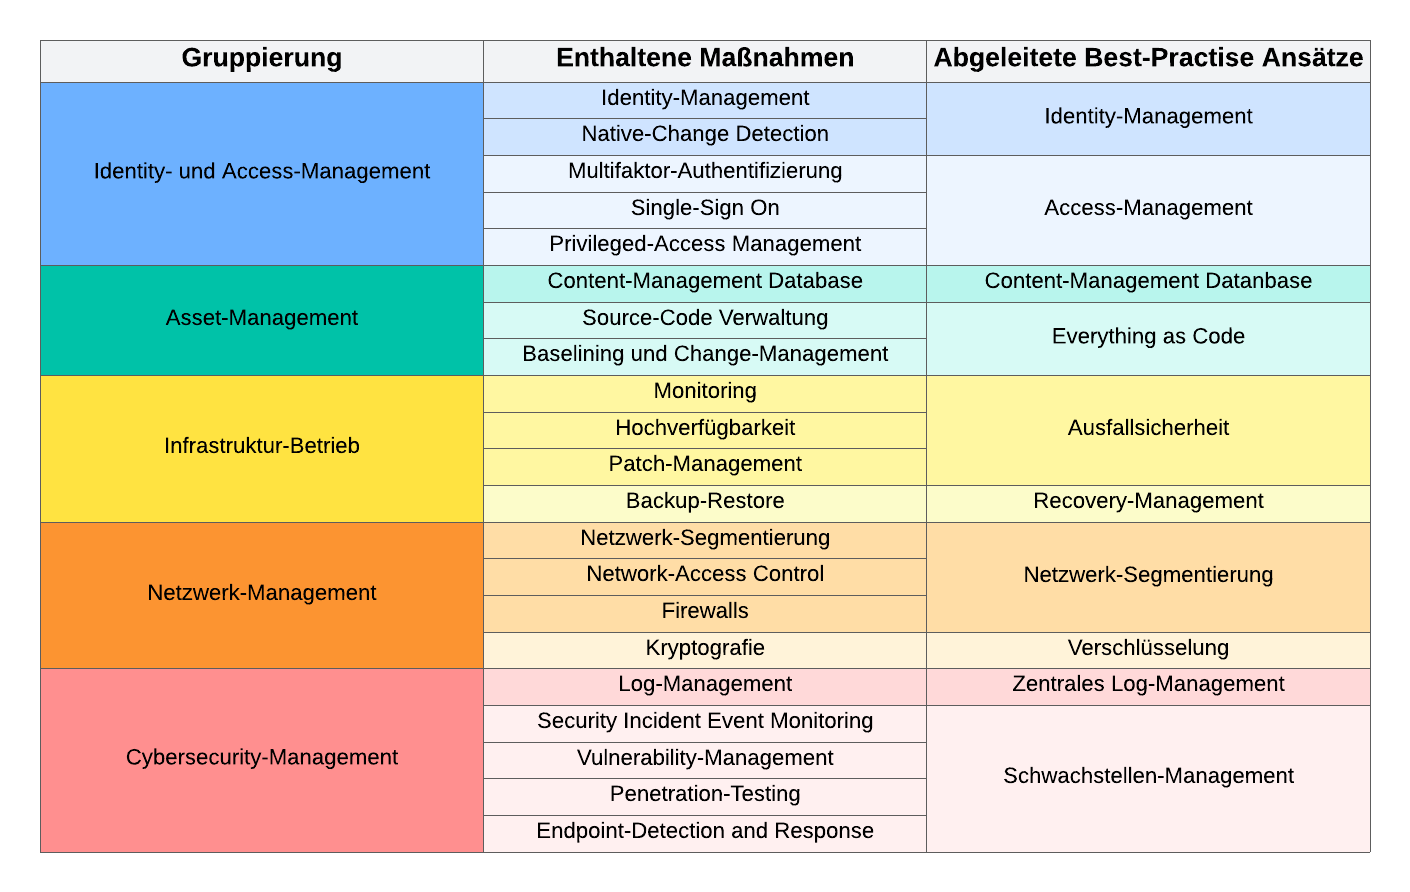
\includegraphics[width=\linewidth]{images/uploads/a_figure_15.png}
  \caption{Visuelle Darstellung der Gruppierungen, enthaltenen Maßnahmen und abgeleiteten Best-Practice-Ansätzen. Quelle: Eigene Darstellung, 2022}
  \label{fig:bp-matrix}
\end{figure}

\section{Identity- und Access-Management}
Die Gruppe \glqq{}Identity- und Access-Management\grqq{} (IAM) vereint die Maßnahmen \glqq{}Identity-Management\grqq{}, \glqq{}Privileged-Access Management\grqq{} (PAM), \glqq{}Multifaktor-Authentifizierung\grqq{} (MFA), \glqq{}Single-Sign On\grqq{} (SSO) und \glqq{}Native-Change Detection\grqq{} (NCD). Die Gruppe beschäftigt sich mit dem Lifecycle, der Authentifizierung und der Autorisierung von Identitäten und Benutzeraccounts.
\bigbreak
Darran Rolls und Morey J. Haber beschreiben in ihrem Buch \glqq{}Identity Attack Vectors: Implementing an Effective Identity and Access Management Solution\grqq{} fünf Grundpfeiler des IAM, die fünf \glqq{}A´s\grqq{} \autocite{rolls_haber_2020}:

\begin{itemize}
    \item Administration
    \item Audit
    \item Analyse
    \item Authentifizierung
    \item Autorisierung
\end{itemize}
\bigbreak
Die in der Gruppe IAM enthaltenen Maßnahmen decken jede für sich einen Teil der fünf A´s ab und tragen so zum Schutz von Identitäten und IT-Systemen bei. 

\subsubsection{Best-Practice-Ansatz: Identity-Management-System (IDM)}
Um Identitäten eines Unternehmens und deren zugeordnete Accounts in den unterschiedlichen Systemen verwalten zu können, ist eine globale Administration von beteiligten Identitäten erforderlich. Die in Kapitel \ref{kap_anforderungsmatrix_abgleitete_maßnahmen} abgeleitete Maßnahme \glqq{}Identity-Management\grqq{} deckt die drei Bereiche \glqq{}Administration\grqq{}, \glqq{}Audit\grqq{} und \glqq{}Analyse\grqq{} ab. Eine globale Administration von Identitäten kann mit Hilfe eines \glqq{}Identity-Management Systems\grqq{} (IDM) realisiert werden. Ein IDM verwaltet Identitäten und bildet den gesamten Lifecycle einer Identität auf Basis von Prozessen ab. Zu diesem Lifecycle zählen das Erstellen der Identität, das Erstellen von Accounts, die Vergabe, Änderung und der Entzug von Berechtigungen. Das Ausscheiden einer Identität aus dem Unternehmen und damit einhergehend das Löschen aller zugehörigen Accounts schließt den Lifecycle ab. Ein IDM bietet somit die Möglichkeit den gesamten Lifecycle einer Identität zu definieren, durchzuführen und zu auditieren. Um dies zu ermöglichen werden unterschiedliche IT-Systeme, in Form von \glqq{}Applikationen\grqq{}, an das IDM angebunden. Beispiele für angebundene Applikationen sind etwa Benutzerdatenbanken auf die von unterschiedlichen anderen IT-Systemen zugegriffen wird. 
\bigbreak
Aufgrund der Tatsache, dass ein IDM System den gesamten Lifecycle von Identität und Berechtigungen abbildet, muss die Integrität der Daten gewährleistet werden. Aus diesem Grund wird ein IDM System als \glqq{}Single Source of Truth\grqq{} etabliert. Eine nicht autorisierte Änderung an einer Identität kann mittels NCD erkannt und behoben werden. Somit wird gewährleistet, dass ein IDM System bei einer direkten, nicht autorisierten Änderung in einem angebundenen System eingreifen kann. Eine mögliche Aktion des IDM wäre, dass die durchgeführte Änderung automatisch überschrieben und somit der vom IDM definierten Stand der Identität wieder herstellt wird. Mittels NCD können Unternehmen der Anforderung Nummer 317 laut Anforderungsmatrix nachkommen. In dieser Anforderung fordert die FMA, dass Unternehmen durch technisch-organisatorische Maßnahmen sicherzustellen haben, dass eine Manipulation der Berechtigungskonzepte verhindert wird.\\

Durch die Abbildung des Lifecycles von Identitäten und Berechtigungen innerhalb eines IDM wird auch weiteren Anforderungen von Aufsichtsbehörden nachgekommen. So ist laut Anforderung Nummer 315 aus der Anforderungsmatrix ein Unternehmen laut FMA verpflichtet, dass die Einräumung, Änderung, Deaktivierung und Löschung von Berechtigungen nachvollziehbar, zuordenbar und auswertbar dokumentiert wird. Diese Anforderung kann mit Hilfe eines IDM realisiert werden.
\bigbreak
Eine weitere Anforderung der FMA besteht darin, dass die den Identitäten eingeräumten Berechtigungen jederzeit, auditierbar sein müssen. Die Anforderung ist in der Anforderungsmatrix unter der Nummer 45 ersichtlich und kann mittels einer Rezertifizierung von Berechtigungen erfüllt werden. Im Zuge einer Rezertifizierung wird überprüft, welche Identitäten ein zu auditierendes Recht besitzen. Somit kann die Zuordnung einer bestimmten Berechtigung im Zuge einer Rezertifizierung legitimiert oder auch sämtlichen Identitäten gesammelt entzogen werden. Auch eine \glqq{}Separation of Duty\grqq{} (SoD) kann mittels eines IDM realisiert werden. Unter einer SoD versteht man eine Funktionstrennung von Identitäten. Mit Hilfe dieser Funktionstrennung soll beispielsweise vermieden werden, dass eine Identität die Berechtigung für das Anfordern eines Darlehens und gleichzeitig die Berechtigung für die Genehmigung dieses Darlehens besitzt. Das Vorhandensein von solchen Konstellationen kann mittels einer Analyse durch ein IDM überprüft werden.
\bigbreak
Ein Beispiel für ein IDM, das die beschriebenen Funktionen zur Verfügung stellt, ist \glqq{}Sailpoint Identity-IQ\grqq{} \autocite{Sailpoint_Identity_IQ}.

\subsubsection{Best-Practice-Ansatz: Access-Management}
Die beiden nach Darran Rolls und Morey J. Haber noch verbleibenden Grundpfeiler \glqq{}Authentifizierung\grqq{} und \glqq{}Autorisierung\grqq{} zählen zum Bereich des Access-Managements. 
\bigbreak
Unter einer Authentifizierung wird ein Login in Verbindung mit einer Art von Geheimnis, meist in der Ausprägung eines Passworts, verstanden. Eine Authentifizierung (v. griechischen \glqq{}authentikos\grqq{} für Urheber, der Echte, der Wirkliche), bezeichnet das Nachweisen einer Identität und den legitimen Zugang zu Privilegien, die der nachgewiesenen Identität zustehen. Alexander Tsolkas und Klaus Schmidt beschreiben in ihrer Arbeit \glqq{}Rollen und Berechtigungskonzepte - Identity- und Access-Management im Unternehmen\grqq{} die Möglichkeit zur Durchführung einer Authentifizierung mittels drei unterschiedlichen Objekten \autocite{TsolkasAlexander2010RuB:}: 

\begin{itemize}
    \item Preisgabe von Wissen (Passwort, PIN-Code, ...)
    \item Benutzung eines Besitzes (Token, ...)
    \item Benutzung des eigenen Subjekts (Retinascan, Fingerabdruck, ...)
\end{itemize}
\bigbreak
Die Authentifizierung einer Identität erfolgt im einfachsten Fall mittels Benutzername und Kennwort und wird von dem jeweiligen System durchgeführt, auf das die Identität zugreifen möchte. Das System nimmt hierfür den Benutzeraccount und das Passwort der Identität entgegen und verifiziert diese beiden Daten gegen eine Datenbank. Diese als \glqq{}Basic-Authentication\grqq{} bekannte Methode hat den Nachteil, dass jedes System für sich eine Abbildung der im IDM verwalteten Identitäten besitzen oder Zugriff auf die zugrunde liegende Datenbank haben muss. Mit der Anzahl der Systeme die Zugriff auf sensible Daten, wie etwa der Datenbank mit Benutzeraccounts und Kennwörtern benötigen, steigt auf das Risiko bei einer Kompromittierung des Systems. Gerade bei Systemen die beispielsweise aus dem freien Internet erreichbar sind oder nicht in der Verantwortung eines Unternehmens stehen, ist ein direkter Zugriff auf Benutzerdaten kritisch zu sehen. \autocite{rolls_haber_2020}
\bigbreak
Die EBA fordert in ihrer Leitlinie für das Management von IKT- und Sicherheitsrisiken, dass Authentifizierungsmethoden der Kritikalität der IKT-Systeme angemessen sein sollen. Diese Anforderung ist unter der Nummer 117 in der Anforderungsmatrix ersichtlich. Auf Basis dieser Anforderungen wurden Möglichkeiten etabliert, damit kritische Systeme nicht mit sensiblen Daten, wie etwa Passwörtern, in Berührung kommen. Eine Möglichkeit dafür bietet die Verwendung von Token-basierten Authentifizierungsmethoden, wie sie bei SSO-Systemen verwendet werden. Das \glqq{}OAuth 2.0 Protokoll\grqq{} beziehungsweise die Verwendung des Layers \glqq{}OpenID-Connect 1.0\grqq{} bietet Verfahren für diese Art der Authentifizierung. OAuth 2.0 ist ein offenes und standardisiertes Protokoll für die Token-basierte Authentifizierung im Internet \autocite{OAUTH2} \autocite{OpenID}. \\\\
Abbildung \ref{fig:token_auth} zeigt den Ablauf einer Authentifizierung mittels Token.  
Im Zuge der Authentifizierung sind drei Komponenten beteiligt. Der \glqq{}Browser\grqq{} symbolisiert die Identität, die Zugriff auf eine Ressource, die \glqq{}Applikation\grqq{} erhalten möchte. Der \glqq{}Authorization Server\grqq{} übernimmt die Rolle des SSO-Systems. Im ersten Schritt fordert der Browser Zugriff auf die Applikation. Innerhalb der Applikation wurde definiert, dass die Authentifizierung über den Authorization-Server stattfinden soll. Aus diesem Grund antwortet die Applikation mit einem Redirect zum Authorization-Server. Im Zuge des Redirects bietet der Authorization-Server eine Login-Seite, auf sich die Identität mittels Benutzername und Kennwort anmeldet. Der Authorization-Server validiert die von der Identität eingegeben Daten und antwortet mit einem Redirect zurück zur Applikation, gepaart mit einem zuvor generierten Authentication-Code. Im nächsten Schritt fordert die Applikation unter Verwendung des Authentication-Codes einen Token beim Authorization-Server an. Nach erfolgreicher Validierung des Authentication-Codes durch den Authorization-Server wird ein Token generiert und der Applikation übermittelt. Der Token stellt somit die Legitimation der Identität sicher. Aufgrund der Tatsache, dass die Applikation dem Authorization-Server vertraut, kann nun der Zugriff auf die Applikation gewährt werden. 
\bigbreak
Dieses Beispiel beschreibt die Möglichkeit einer Anmeldung an einem kritischen System. Der Vorteil liegt darin, dass das System selbst zu keinem Zeitpunkt der Anmeldung Kenntnis über die Logindaten der Identität erhält.

\begin{figure}[H]
    \centering
  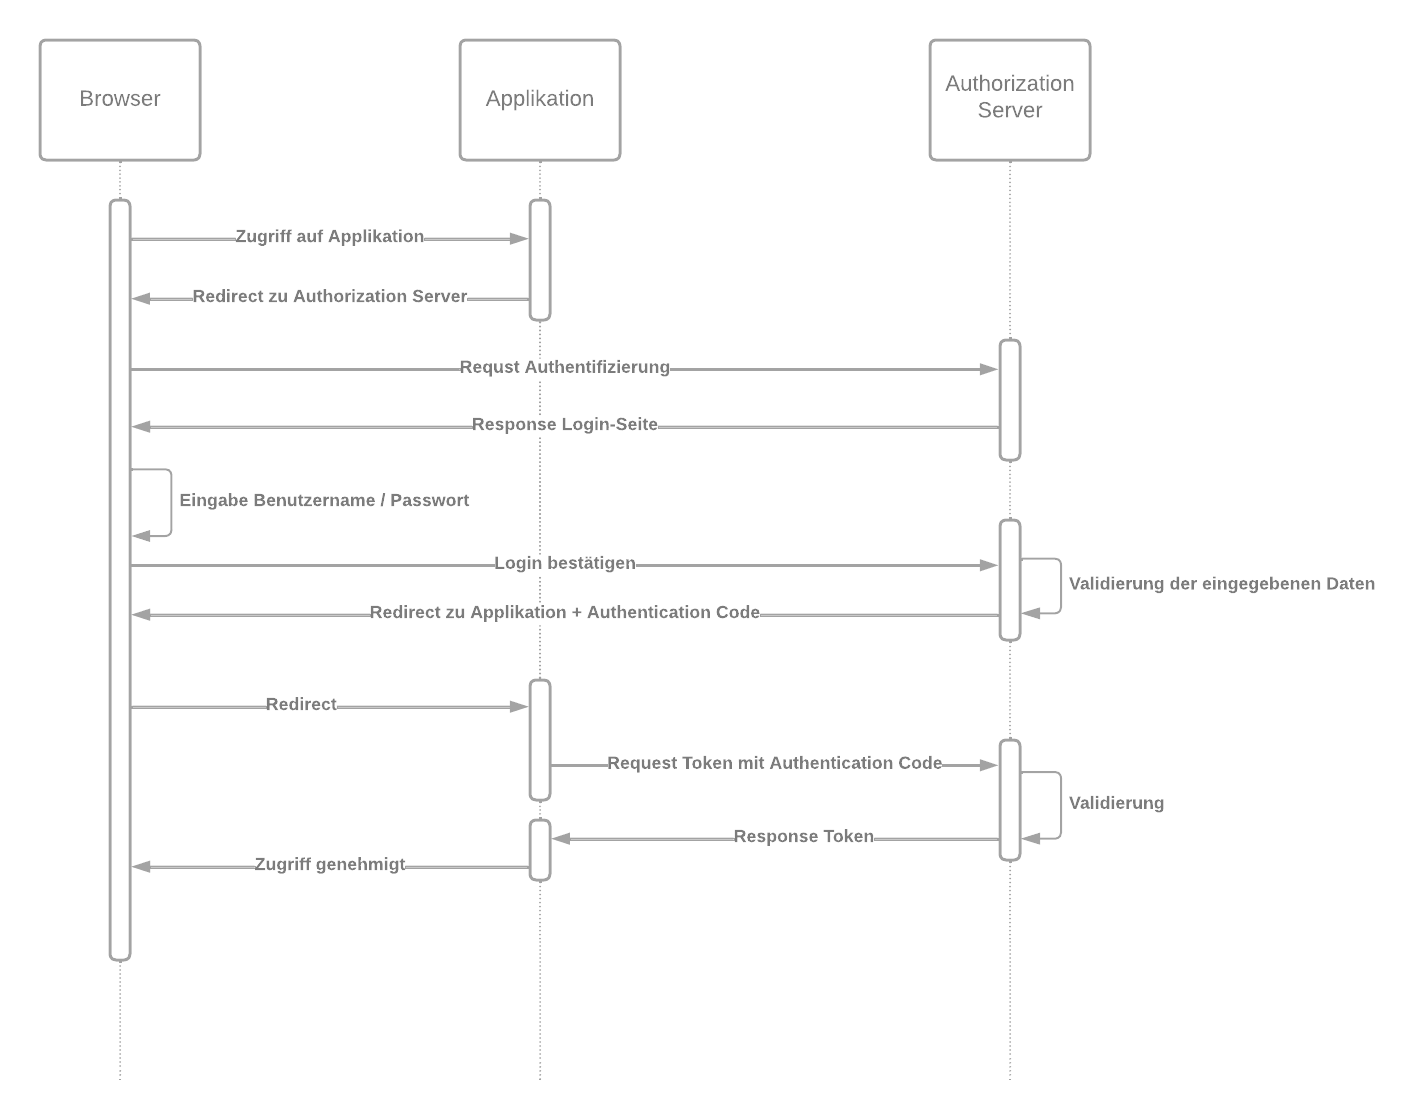
\includegraphics[width=\linewidth]{images/uploads/a_figure_06.png}
  \caption{Visuelle Darstellung einer Authentifizierung mittels Token. Quelle: Eigene Darstellung, 2022}
  \label{fig:token_auth}
\end{figure}

Die Authentifizierung über SSO kann hierbei noch um die Verwendung zusätzlicher Faktoren abgesichert werden. So benötigt eine Identität im Zuge der Authentifizierung neben dem Kennwort einen oder mehrere zusätzliche Faktoren, wie etwa einen zufällig generierten Code oder dem Vorhandensein einer Chip-Karte. MFA wird von vielen gängigen SSO-Frameworks, wie etwa \glqq{}Redhat Single Sign-On\grqq{} unterstützt \autocite{RedHat_SSO}. 
\bigbreak
Das Thema Access-Management bietet unterschiedliche Ausprägungen mit denen sich der Schutz von Identitäten und IT-Systemen verbessern lässt. PAM ist eine Subdisziplin im Bereich des IAM und eine Methode um privilegierte Aktivitäten auf Ressourcen abzusichern, zu kontrollieren, zu Monitoren und zu Managen. Unter einem privilegierten Account versteht man Accounts, die über besondere Berechtigungen verfügen. Beispiele hierfür sind lokale Administratoren, Service-Accounts, Domänen-Administratoren, privilegierte User-Accounts und C-Level Accounts. Das Ziel von PAM ist eine Risikominimierung, in dem privilegierter Zugriff auf Ressourcen nur dann gewährt wird, wenn die Notwendigkeit dafür besteht. Auf diese Weise wird vermieden, dass privilegierte Accounts während der täglichen Arbeit verwendet werden oder diese von Angreifern ausgenutzt werden können. Letzteres wird dadurch gewährleistet, dass Kennwörter für privilegierte Accounts erst bei Anforderung generiert werden. Abbildung \ref{fig:best-practice PAM} zeigt einen Möglichen Ablauf für den Zugriff auf eine Ressource durch einen Administrator unter der Verwendung von PAM. Es ist zu erkennen, dass der privilegierte Zugriff auf eine Ressource on-demand angefordert und von einem Dritten genehmigt werden muss. Der privilegierte Zugriff wird nach Beendigung des Task oder nach einem zuvor definierten Zeitraum automatisch entfernt. \autocite{rolls_haber_2020} 

\begin{figure}[H]
    \centering
  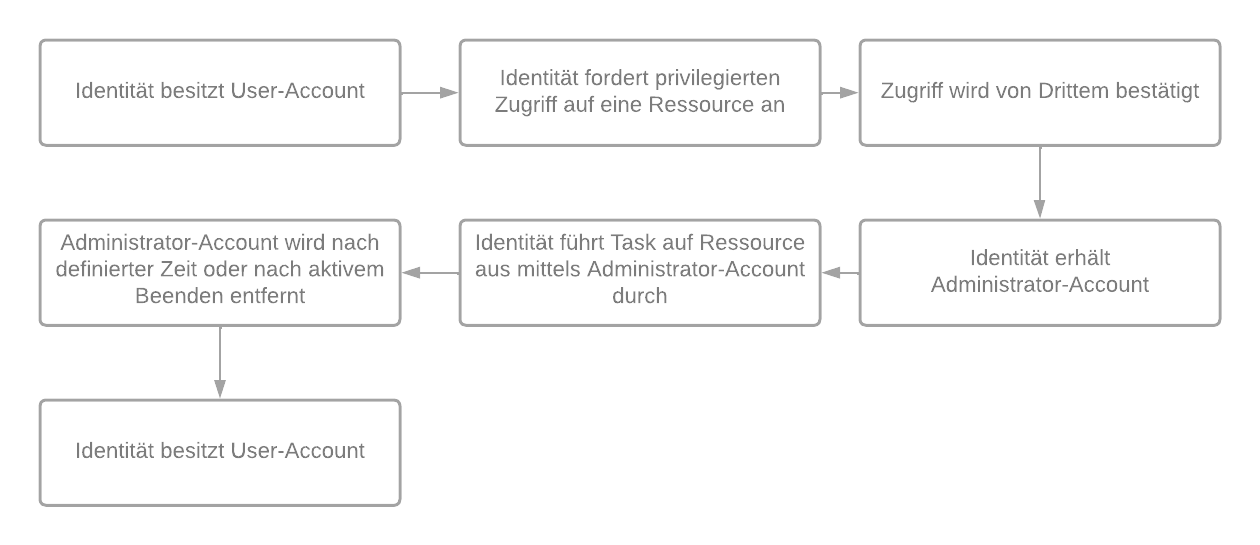
\includegraphics[width=\linewidth]{images/uploads/a_figure_07.png}
  \caption{Visuelle Darstellung des Zugriffs auf eine Ressource mittels PAM. Quelle: Eigene Darstellung, 2022}
  \label{fig:best-practice PAM}
\end{figure}

Mit Hilfe von PAM kann das \glqq{}Least-Privilege\grqq{} Modell, das Prinzip der minimalen Rechtevergabe realisiert werden. Dieses Prinzip wird sowohl von der EBA als auch von der BaFin gefordert. Die Anforderungen sind in der Anforderungsmatrix unter Nummer 41 und Nummer 111 hinterlegt. 
\bigbreak
Die beiden Best-Practice-Ansätze und die jeweiligen technischen Umsetzungen SSO, MFA, NCD und PAM adressieren die von Darran Rolls und Morey J. Haber beschriebenen Grundpfeiler der Authentifizierung und Autorisierung und decken die von Aufsichtsbehörden gesetzten Anforderungen aus dem Bereich IAM ab. 

\section{Asset-Management}
Die Gruppe \glqq{}Asset-Management\grqq{} vereint die Maßnahmen \glqq{}Content-Management\\-Database\grqq{}, \glqq{}Source-Code-Verwaltung\grqq{} und \glqq{}Baselining und Change-Management\grqq{}. Die Gruppe beschäftigt sich mit der Dokumentation, Sicherung, Änderung und Bereitstellung von Asset-Daten. 
\bigbreak
Eine zentrale und konsistente Übersicht über den aktuellen Zustand der gesamten IT-Umgebung ist ein wesentlicher Grundstein für einen reibungslosen Betrieb und die Implementierung und Sicherstellung der IT-Sicherheit im Unternehmen. Aus diesem Grund fordert die EBA, dass Unternehmen eine Übersicht über eigene IT-Assets und IKT-Systeme besitzen und diese Übersicht stets aktuell zu halten haben. Des Weiteren sind Unternehmen verpflichtet ein aktuelles Verzeichnis über die eigenen IKT-Assets zu führen und deren Verbindungen und Abhängigkeiten zueinander darzustellen. Diese beiden Anforderungen sind in der Anforderungsmatrix unter Nummer 97 und Nummer 136 ersichtlich. Die FMA fordert Abhängigkeiten von IT-Systeme abzubilden, das IT-Inventar zu verwalten und entsprechend zu steuern (Anforderungsmatrix Nummer 275). Die BaFin fordert, dass Unternehmen jederzeit einen aktuellen Überblick über die Bestandteile des festgelegten Informationsverbunds und deren Abhängigkeiten geben können. Außerdem muss die Geschäftsleitung imstande sein Aussagen zu selbst betriebenen IT-Systemen treffen zu können. Die Anforderungen der Bafin sind in der Anforderungsmatrix unter Nummer 5 und Nummer 7 ersichtlich. 

\subsubsection{Best-Practice-Ansatz: Configuration Management Database}
Eine \glqq{}Configuration Management Database\grqq{} (CMBD) ist eine Möglichkeit um den Anforderungen der Aufsichtsbehörden in diesem Bereich nachzukommen. Eine CMDB unterstützt Unternehmen dabei stets einen aktuellen Überblick über alle IT-Systeme, aktuelle Konfigurationen und betriebenen Services zu erhalten. Des Weiteren bildet eine CMDB die Grundlage für unterschiedliche IT-Sicherheitssysteme und nach gelagerte Automatisierungswerkzeuge, die auf Basis der von der CMDB bereit gestellten Daten arbeiten. Eine CMDB aggregiert die Datenbestände unterschiedlicher Systeme, korreliert diese und wertet sie aus. 
\bigbreak
Für eine optimale Darstellung der IT-Landschaft ist die zugrunde liegende Datenqualität von höchster Priorität. Die benötigten Konfigurationsdaten der einzelnen IT-Systeme manuell zu erheben gestaltet sich mit steigender Komplexität der IT-Infrastruktur unwirtschaftlich bis hin zu unmöglich. Für die Aggregation der Daten können automatische Discovery-Tools unterstützen. Ein Beispiel hierfür sind \glqq{}Endpoint-Detection and Response Systeme\grqq{} (EDR) wie Tanium\footnote{https://www.tanium.com}, die auf allen IT-Assets installiert werden. Mit Hilfe von Tanium können Echtzeitdaten der IT-Assets ausgelesen und an die CMDB übermittelt werden. Ein weiterer Vorteil von Tanium besteht darin, dass auch IT-Assets auf denen Tanium nicht installiert werden kann, erkannt werden können. Beispiele hierfür sind Netzwerk-Komponenten oder Appliance-Lösungen. Tanium erkennt und analysiert diese Systeme auf Basis der Verbindungen zu Systemen auf denen Tanium bereits installiert wurde. 
\bigbreak
Trotz der Verwendung von Tools wie Tanium können physikalische Komponenten in Unternehmen betrieben werden, nicht nicht automatisch erkannt werden können. Hier ist die Einbindung in Prozesse wie dem Change-Management relevant um einen stets aktuellen und konsistenten Datenbestand zu erhalten. Eine CMDB kann neben der technischen Daten eines IT-Assets noch weitere Informationen enthalten. So kann die Beschreibung eines IT-Assets aus folgenden Komponenten bestehen:

\begin{itemize}
    \item Technische Daten
    \begin{itemize}
        \item IP-Adresse
        \item MAC-Adresse
        \item CPU, RAM, ...
    \end{itemize}
    \item Geografischer Standort
    \item Betriebssystem
    \begin{itemize}
        \item Version
        \item Lizenzkey
        \item Lizenzvertrag
    \end{itemize}
    \item Seriennummer
    \item Inventarnummer
    \item Servicevertrag
    \item SLA-Level
    \item Applikationen
    \item Sonstige Dokumente
\end{itemize}
\bigbreak
Anhand dieser Informationen lässt sich auf Basis unterschiedlicher Informationsquellen ein Gesamtbild der IT-Infrastruktur erstellen und den Anforderungen von Aufsichtsbehörden nachkommen.

\subsubsection{Best-Practice-Ansatz: Everything as Code (EaC)}
Auch in Bezug auf die Nachvollziehbarkeit von Änderungen an Assets werden Anforderungen gestellt. Die EBA und die BaFin fordern, dass Organisationen die Integrität der Anwendungen und Systeme angemessen sicherzustellen haben. Des Weiteren müssen Vorkehrungen getroffen werden um versehentliche Änderungen oder absichtliche Manipulationen erkennen zu können. Diese Anforderungen sind in der Anforderungsmatrix unter den Nummern 54 und 125 ersichtlich. Unternehmen sind laut BaFin außerdem dazu verpflichtet, Änderungen an IT-Systemen in geordneter Art und Weise aufzunehmen, zu dokumentieren, zu bewerten, zu genehmigen und zu koordinieren (Anforderungsmatrix Nummer 63). Laut EBA sind Konfigurationsbaselinies für alle Netzwerkkomponenten zu implementieren.
\bigbreak
EaC ist eine Technik, in der sämtliche Teile eines Systems als Code behandelt werden. Dieses Prinzip wird bereits verstärkt im Bereich der Softwareentwicklung verwendet, wo sämtlicher Source-Code in Repositories wie etwa Apache-SVN\footnote{https://subversion.apache.org} oder Github\footnote{https://github.com} verwaltet wird, um eine SoT zu definieren. SoT beschreibt ein Konzept, in dem Daten von unterschiedlichen Systemen eines Unternehmens in einem bestimmten Platz aggregiert werden um Datensilos zu vermeiden. So wird sichergestellt, dass Systeme Daten von nur einer Quelle beziehen, welche stets den aktuellen Stand widerspiegelt. Ein \glqq{}Code-Repository\grqq{} (CR) ist der erste Schritt in der Deployment-Pipeline vom Source-Code hin zum fertigen Produkt oder System. Im Zuge des Deployment-Prozesses werden unterschiedliche Schritte, wie etwa automatische Tests oder automatische Freigabeprozesse in der Pipeline durchgeführt. Ein CR bildet somit einen Baustein für die von den Aufsichtsbehörden definierten Anforderungen. \autocite{mulesoft}
\bigbreak
Gerade mit der Etablierung der DevOps Bewegung, in der sich die Bereiche „Software-Development“ und „IT-Operations“ zusammenschließen, um einen sicheren, effizienteren und vor allem automatisierten System-Lifecycle zu definieren, nimmt die Vorgehensweise der Behandlung von Komponenten als Code, neben der Softwareentwicklung auch verstärkt Einzug in anderen Bereiche der IT. \autocite{könig_kugel_2019}
\bigbreak
Einer dieser Bereiche ist die IT-Infrastruktur, in der sich der Grad der Automation häufig auf wieder ausführbare Skripte oder speziell angepasste Betriebssystem-Images begrenzt. Darüber hinausgehende Konfigurationen werden manuell oder mit Skripten, welche eigens für den jeweiligen Server angepasst werden, durchgeführt. \glqq{}Infrastructure as Code\grqq{} (IaC) übernimmt die Bereitstellung und die Konfiguration der gesamten Infrastruktur im Quellcode und ermöglicht das Schaffen von konsistenten und wiederholbaren Routinen. \autocite{özel_pautz_schmidt_2020}
\bigbreak
Unterschiedliche Anbieter von Container Virtualisierungslösungen, wie etwa Docker\footnote{https://www.docker.com} oder Redhat-Openshift\footnote{https://www.openshift.com}, arbeiten bereits mit einheitlichen Konfigurationen, welche Server oder Applikationen auf Basis von Templates beschreibend definieren, um diese so vom jeweiligen Framework plattformunabhängig provisionieren zu lassen. Weitere wichtige Themen, die eng mit dem Provisioning von Servern oder Applikationen verbunden sind werden häufig separat in anderen Tools behandelt oder gar nicht berücksichtigt. Zu diesen Themen zählen unter anderem das Erstellen von Dokumentationen, dem Berücksichtigen und Auditieren von Berechtigungsfreigaben oder dem Einpflegen und Berücksichtigen von IT- Sicherheitsrichtlinien.
\bigbreak
Einen weiteren Bereich, der von der Behandlung von Komponenten als Code profitieren kann, bildet der Compliance-Bereich, die Einhaltung von Governance-Richtlinien. Mit Hilfe von \glqq{}Policy as Code\grqq{} (PaC) wird versucht bei der Überprüfung auf Richtlinien weg von einem manuellen Ansatz der von Menschen durchgeführt wird, hin zu einem konsistenten, effizienten und wiederholbaren Ansatz der Überprüfung von Richtlinien, auf Basis von Code zu kommen. \autocite{hashicorp_policyascode}
\bigbreak
Der Zusatz \glqq{}as Code\grqq{} weist auf die der jeweiligen Technologie hinzugefügten Attribute Effizienz, Sicherheit, Transparenz und Automatisierung hin und versucht diese Themen ebenso im Zuge des Provisionings zu berücksichtigen. Spricht man von \glqq{}codification\grqq{} bedeutet dies den Erhalt von automatisierten Tests, einer einheitlichen Sprache, welche sowohl von IT-affinen als auch Mitarbeiter aus dem organisatorischem Umfeld verstanden werden kann, und einer automatisierter Deployment-Pipeline, welche sich modular um diverse Komponenten erweitern lässt. Eine Deployment-Pipeline beschreibt den automatisierten Prozess von der Erstellung des Quellcodes bis hin zum Provisioning des fertigen Produkts. Mit Hilfe unterschiedlicher Schritte ermöglicht eine Deployment-Pipeline die automatisierte Ausführung von Arbeitsschritten. Zu diesen Arbeitsschritten zählen unter anderem eine Versionierung des Quellcodes, eine automatisierte Freigabe von Änderungen, die Ausführung von Tests, das Deployment in eine Test-Umgebung und das anschließenden Deployment in die produktive Umgebung. \autocite{könig_kugel_2019}
\bigbreak
Auf Basis der Vorteile der Definition von Komponenten als Code, gliedert sich der Bereich EaC unter anderem in folgende Teilbereiche:
\begin{itemize}
    \item Infrastructure as Code
    \item Security as Code
    \item Policy as Code
\end{itemize}
\bigbreak
\textbf{Infrastructure as Code}\\
Mit Hilfe von IaC können die Anforderungen der BaFin und der EBA in Bezug auf Änderungen an Assets unter Einbezug eines Genehmigungsprozesses und der Etablierung von Konfigurationsbaselines nachgekommen werden. 
IaC versucht die Vorteile von EaC bezogen auf Infrastrukturkomponenten zu behandeln und abzudecken. Sämtliche Teile eines Systems, wie etwa die Konfiguration der virtuellen Umgebung, die Konfiguration des Betriebssystems, Einstellungen betreffend installierter Programme oder auch die Dokumentation dieser, werden in Repositories gespeichert.
Dies bringt unter anderem folgende Vorteile mit sich \autocite{hackernoon_2020}:
\begin{itemize}
    \item Nachvollziehbarkeit\\
        Änderungen an Systemen können jederzeit detailliert nachvollzogen oder rückgängig gemacht werden. Backups und Restores von Infrastrukturkomponenten sind großteils überflüssig, da die Komponenten ad-hoc neu provisioniert werden können.
    \item Wiederholbarkeit\\
        Systeme können jederzeit auf unterschiedliche Plattformen provisioniert werden (Ready for Cloud). Somit bietet IaC die Möglichkeit einer \glqq{}On Demand Infrastruktur\grqq{}.
    \item Testing\\
        Durch ein Testing Verfahren können Änderungen am System getestet und bei erfolgreichem Test automatisiert in der Produktionsumgebung provisioniert werden.
    \item Schutz vor Server- und Configuration Drift\\
        Es existiert nur mehr eine SoT. Änderungen, welche direkt am Zielsystem vorgenommen und somit nicht in der SoT aufzufinden sind, werden automatisch überschrieben. Dies dient zum einen dem Erkennen von unautorisierten Änderungen von Einstellungen am System, zum anderen beugt es Configuration-Drifts vor. Darunter versteht man das Abweichen einer Konfiguration von einem definierten und gewünschten Zustand. Configuration-Drifts können etwa entstehen, wenn unterschiedliche Server von verschiedenen Mitarbeitern erstellt und konfiguriert werden. Obwohl alle Mitarbeiter nach denselben Vorgaben arbeiten, können sich Unterschiede in der Konfiguration ergeben. \autocite{morris}
    \item Dokumentation und Geteiltes Wissen\\
        Sämtliche Komponenten eines Systems werden an einer gesammelten Stelle dokumentiert und sind dort einsehbar. Arbeiten mehrere Personen, oder sogar unterschiedliche Teams, an ein und demselben System, kann das Wissen durch eine einheitliche Definitionssprache leichter vermittelt und die verwalteten Systeme schneller erfasst werden. Auch personellen Ausfällen kann so vorgebeugt werden. Bei Standalone-Lösungen kann es Mitarbeitern ohne einer vorhandenen Dokumentation Probleme bereiten, die ursprüngliche Intention des Erstellers oder manuelle Änderungen an einem System nachzuvollziehen.
    \item Freigabe und Audit\\
        Änderungen am System, ohne vorheriger Freigabe durch das Management, werden technisch unterbunden. Durch die zentrale Speicherung sämtlicher Komponenten eines Systems, werden etwaige Audit-Anfragen und Feedback-Schleifen signifikant beschleunigt.
\end{itemize} 
\bigbreak
Der Vollständigkeit halber wird auch noch auf die beiden anderen Teilbereiche von EaC eingegangen. Obwohl die Anwendungsgebiete von \glqq{}Security as Code\grqq{} (SaC) und \glqq{}Policy as Code\grqq{} (PaC) nicht explizit von den Aufsichtsbehörden gefordert sind, tragen sie dennoch stark zu einer sicheren und stabilen IT-Infrastruktur bei. 
\bigbreak
\textbf{Security as Code}\\
SaC beschreibt Techniken um Sicherheit bei der Entwicklung mittels einer Deployment-Pipeline zu gewährleisten. Im Zuge des jeweiligen Deployment-Prozesses werden automatisiert Sicherheitsüberprüfungen durchgeführt und nach Schwachstellen gesucht.
Folgende Überprüfungen können als Teil einer zusätzlichen Sicherheitsschicht integriert werden \autocite{hackernoon_2020}:
\begin{itemize}
    \item Automatische Vulnerarbility-Scans
    \item Ausführung von Skript-Tests
    \item Überprüfung auf Default-Konfigurationen
    \item Implementierung von Monitoring Funktionalitäten
\end{itemize}
\bigbreak
Diese Ansätze bringen unter anderem folgende Vorteile mit sich \autocite{hackernoon_2020}:
\begin{itemize}
    \item Schnellere Reaktion auf Änderungen und Sicherheitsanforderungen
    \item Bessere Zusammenarbeit zwischen den einzelnen Teams
    \item Vulnerabilities können in einem frühen Stadium erkannt und behoben werden
    \item Entwicklungskosten können durch das automatisierte und frühzeitige Erkennen von
    Schwachstellen und Fehlern verringert werden
    \item Die Möglichkeit für automatisierte Sicherheitsüberprüfungen wird geschaffen
\end{itemize}
\bigbreak
\textbf{Policy as Code}\\
PaC beschreibt die Möglichkeit Richtlinien in einem Weg zu definieren, dass diese sowohl von Mensch als auch Maschine gelesen, interpretiert und validiert werden können.
Das Ziel von PaC ist es organisatorische Richtlinien des Unternehmens automatisch zu implementieren, verifizieren, monitoren und zu reporten. Ein großer Vorteil besteht darin, dass Richtlinien bereits im Zuge des Deployment-Prozesses behandelt werden können. So wird gewährleistet, dass bereits während der Entwicklung frühzeitig und nachvollziehbar auf potentielle Policy-Verletzung reagiert werden kann.

Um PaC zu ermöglichen können die jeweiligen Richtlinien auf Basis von Code abgebildet und in Form von Tests in den Deployment-Prozess integriert werden. Ein weiterer Weg ist, Richtlinien mit der Konfiguration der Deployment-Pipeline durchzusetzen. Auf diesem Weg können etwa unterschiedliche Aktionen oder Abläufe unterbunden werden. PaC baut somit automatisierte Compliance sowohl in der Entwicklung als auch im Betrieb auf.
Der Begriff „Policy“ ist in der Literatur nicht klar definiert und umfasst mehrere Bereiche \autocite{dadgar}:
\begin{itemize}
    \item Compliance Policies\\
    Diese Richtlinien schaffen Compliance unter Einbezug externer Standards wie
    dem „Payment Card Industry Security Standard“ (PCI-DSS5) oder der „General Data Protection Regulation“ (GDPR6) \autocite{PCIDSS5} \autocite{GDPR}.
    \item Security Policies\\
    Diese Richtlinien definieren interne Datenschutz- und Datensicherheits-Vorgaben eines Unternehmens um die Sicherheit und die Integrität von Daten zu schützen. Die Definition von Applikationen, welche vom freien Internet aus erreichbar sind, stellen ein Beispiel für eine Security Policy.
    \item Operational Excellence\\
    Diese Art von Policy verhindert Service-Ausfälle oder Service-Verschlechterungen zu Lasten des Unternehmens oder des Kunden. Beispiele hierfür sind die Validierung von neuen Konfigurationseinstellungen oder die Sicherstellung einer redundant ausgelegten Anbindung von Systemen.
\end{itemize}
\bigbreak
Die Definition von Richtlinien mittels PaC bietet unter anderem folgende Vorteile \autocite{hackernoon_2020}:
\begin{itemize}
    \item Routineberichte optimieren die Auditierung von Systemen\\
    Berichte, die während des gesamten DevOps-Lebenszyklus generiert werden liefern Dokumentation und Nachweis, mit deren Hilfe viele internen und behördlichen Prüfungsverfahren nachverfolgt und rationalisiert werden können.
    \item Compliance Transparenz
    \item Zeitersparnis
    \item Kontinuierliche Auditierbarkeit
\end{itemize}

\section{Infrastruktur-Betrieb}
\label{Patch-Management}
Die Gruppe \glqq{}Infrastruktur-Betrieb\grqq{} vereint die Maßnahmen \glqq{}Monitoring\grqq{}, \glqq{}Hochverfügbarkeit\grqq{}, \glqq{}Backup-Restore\grqq{} und \glqq{}Patch-Management\grqq{}. Die Gruppe beschäftigt sich mit der Aufrechterhaltung und der Absicherung von IT-Systemen um einen sicheren und stabilen Betrieb zu gewährleisten. 
Aufsichtsbehörden stellen unterschiedliche Anforderungen an den Betrieb und die Verfügbarkeit von IT-Systemen von Banken. Die BaFin fordert, dass Konzepte zur Hochverfügbarkeit implementiert, angewendet und entsprechend überprüft werden (Anforderungsmatrix Nummer 82). Die EBA fordert, dass Unternehmen Leistungs-. Kapazitätsplanungs- und Kapazitätsüberwachungs-Prozesse einführen um bedeutende Leistungsprobleme von IKT-Systemen und Engpässe bei IKT-Kapazitäten rechtzeitig zu erkennen und darauf reagieren zu können (Anforderungsmatrix Nummer 139). Die FMA setzt des Weiteren voraus, dass die Kontinuität und Ausfallsicherheit der IT-Systeme laufend überprüft und eine rechtzeitige Wiederherstellung von IT-Systemen nach Betriebsausfällen gewährleistet wird (Anforderungsmatrix Nummer 340). Außerdem werden Anforderungen an Update-Prozesse von Systemen gestellt. Die BaFin setzt voraus, dass Unternehmen IT-Systeme regelmäßig aktualisieren und die Stabilität der Systeme im Falle einer Änderung entsprechend testen (Anforderungsmatrix Nummer 61). Im Falle eines Ausfalls oder eines Datenverlustes setzt die EBA voraus, dass Unternehmen Verfahren zur Sicherung und Wiederherstellung von Daten und IKT-Systemen festlegen und umsetzen, um sicherzustellen, dass diese bei Bedarf wiederhergestellt werden können (Anforderungsmatrix Nummer 140). 
\bigbreak
Betrachtet man die Anforderungen der Aufsichtsbehörden, ergeben sich zwei Bereiche die von Banken in Österreich adressiert werden müssen \autocite{kharod_2021}:
\begin{itemize}
    \item Gewährleistung des stabilen Betriebs der IT-Infrastruktur (Ausfallsicherheit)
    \begin{itemize}
        \item Hochverfügbarkeit
        \item Monitoring
        \item Patch-Management
    \end{itemize}
    \item Reaktion auf Ereignisse betreffend IT-Infrastrukturkomponenten (Recovery Management)
    \begin{itemize}
        \item Backup-Restore
    \end{itemize}
\end{itemize}

\subsubsection{Best-Practice-Ansatz: Ausfallsicherheit}
Ist ein System \glqq{}hochverfügbar\grqq{} bedeutet das, dass das System lange Zeit ohne Unterbrechung stabil läuft. Die Verfügbarkeit eines Systems wird in Prozent gemessen. Besitzt ein System eine Verfügbarkeit von 100\%, ist keine Ausfallzeit zu erwarten. In der Realität kann eine Verfügbarkeit von 100\% nahezu ausgeschlossen werden. 
\bigbreak
Eine hochverfügbare Infrastruktur charakterisiert sich unter anderem durch folgende Eigenschaften:
\begin{itemize}
    \item Vermeidung von Single Points of Failure (SPoF)
    \item Redundanz / Load-Balancing
    \item Auto-Skalierbarkeit
    \item Monitoring
\end{itemize}
\bigbreak
SPoFs können in unterschiedlicher Ausprägung bestehen und stellen ein Bottleneck in der Ausfallsicherheit dar. Egal ob es sich bei der Instanz um einen einzelnen Server oder um ein ganzes Rechenzentrum handelt, fällt ein SPoF aus, hat dies Auswirkungen auf alle angebundenen IT-Systeme. 
\bigbreak
Hardware Redundanz wird erzielt in dem zwei oder mehr Instanzen einer Hardware Komponente bereitgestellt werden. Wird zusätzlich ein Load-Balancer implementiert, kann dieser die Last gleichmäßig auf die redundanten Hardware Komponenten verteilen, Lastspitzen abgefangen und die Systemstabilität gewährleisten. Eine weitere Möglichkeit um Lastspitzen abzufangen und auf steigende Auslastung zu reagieren ist die Skalierung von Systemen. Unter einer Auto-Skalierbarkeit versteht man die Fähigkeit von Systemen sich wachsenden oder schrumpfenden Anforderungen hinsichtlich der Leistungsfähigkeit automatisch anzupassen. Es wird zwischen der vertikalen Skalierung (scale up) und der horizontalen Skalierung (scale out) unterschieden. Bei der vertikalen Skalierung wird Leistung innerhalb des IT-Systems hinzugefügt oder entfernt. Die Leistungssteigerung entsteht somit durch das Hinzufügen zusätzlicher Komponenten wie etwa Speicherplatz, CPUs oder zusätzlicher Grafikkarten. Bei der horizontalen Skalierung wird die Leistungssteigerung eines IT-Systems durch das Hinzufügen zusätzlicher Systeme erbracht. Die vom IT-System durchzuführenden Arbeiten wird auf unterschiedlichen Instanzen verteilt. So kann gewährleistet werden, dass steigender Workload mit gleichbleibender Performance abgearbeitet werden kann. \autocite{geißler_2019}
\bigbreak
Um die Stabilität von IT-Systemen gewährleisten und auf etwaige Störungen oder Lastspitzen entsprechend reagieren zu können, ist eine Überwachung der IT-Infrastruktur unumgänglich. \\
Bevor eine Überwachung implementiert wird, sollten folgende Punkte geklärt sein \autocite{ashutosh_nivedita_2022}:
\begin{itemize}
    \item Grund für das Monitoring\\
    Je nach Anwendungsfall kommen unterschiedliche Lösungen für ein Logging und ein Monitoring in Frage. Mögliche Gründe für ein Monitoring sind Compliance-Anforderungen, Gesetzliche Anforderungen oder Incident-Response-Anforderungen. 
    \item Daten, die für das Monitoring benötigt werden\\
    Für das Monitoring von Finanztransaktionen sind beispielsweise andere Daten sinnvoll und nötig, als für das Monitoring von Netzwerk-Komponenten. Unabhängig vom Anwendungsfall sollten Logeinträge folgende Informationen enthalten:
    \begin{itemize}
        \item Durchführender (Wer: Accountname oder IP-Adresse)
        \item Aktion (Was: Lesen/schreiben auf welcher Ressource)
        \item Zeitpunkt (Wann: Timestamp)
        \item Lokation (Wo: Geolocation, Browser, Skript-Name, ...)
    \end{itemize}
    \item Zu überwachende Assets\\
    Um zu verhindern, dass Logdaten die für das Monitoring nötig sind zu viel Speicherplatz in Anspruch nehmen, sollte im Vorfeld geklärt werden welche Assets zu überwachen sind. Basierend auf den jeweiligen Assets ist zu definieren, welche Software-Komponente überwacht werden soll und welcher Daten-Klassifizierung die gesammelten Daten entsprechen.
    \item Sicherheitsaspekt betrachten\\
    Basierend auf der Daten-Klassifizierung sind entsprechende Sicherheitsvorkehrungen zu treffen. Personenbezogene Daten sollten maskiert oder anonymisiert werden. Die Übertragung von Log-Daten sollte verschlüsselt stattfinden und der Zugriff auf den Zustand eines Systems oder einer Applikation einem rollenbasierten Berechtigungskonzept unterliegen.
    \item Automatisierung und Standardisierung\\
    Soweit möglich sollte ein Monitoring automatisiert stattfinden und das System im Fehlerfall automatisch die zuständige Person benachrichtigen. Um Monitoring-Alarme weiterverarbeiten zu können, sollten diese in einem standardisierten Format, etwa im Format \glqq{}JSON\grqq{} übergeben werden \autocite{JSON}.  
\end{itemize}

\bigbreak
Dies Überwachung von IT-Systemen kann mit unterschiedlichen Software-Produkten umgesetzt werden. Die Implementierung einer Monitoring-Software gestaltet sich vergleichsweise einfach. Eine viel größere Herausforderung bietet die Frage, welche Daten im speziellen betrachtet werden müssen um die Instabilität oder Auslastung von IT-Systemen zu erkennen. Um den Gesundheitsstatus eines Systems zu messen werden unterschiedliche Metriken definiert und auf den Systemen gemessen. Unter einer Metrik wird ein Datensatz verstanden, der die Performance und Verfügbarkeit von Ressourcen widerspiegelt. Mit Hilfe von Metriken kann der Status eines Systems zu einer bestimmten Zeit gemessen und entsprechend interpretiert werden. \autocite{geißler_2019} 
\bigbreak
Datadog\footnote{https://www.datadoghq.com}, ein Betreiber von Software-as-a-Service Monitoring Diensten teilt Metriken in die zwei Kategorien \glqq{}Work-Metrics\grqq{} (WM) und \glqq{}Ressource-Metrics\grqq{} (RM). WM geben den Top-Level Status eines IT-Systems an, in dem die Leistung des Systems, bezogen auf die durchzuführende Tätigkeit gemessen wird. 
\bigbreak
WM lassen sich in vier Typen einteilen \autocite{le-quoc_2015}:
\begin{itemize}
    \item Throughput\\
    Gibt die Menge an Tasks an, die das System pro Zeiteinheit absolviert.
    \item Success\\
    Repräsentiert die Anzahl erfolgreich durchgeführter Tasks in Prozent.
    \item Error\\
    Repräsentiert die Anzahl an Fehlern, die ein System während der Durchführung von Tasks produziert.
    \item Performance\\
    Gibt die Effizienz des Systems im Zuge der Durchführung von Tasks an. 
\end{itemize}
\bigbreak
WM können dabei unterstützen eine generelle Aussage zum Status und der Performance eines Systems zu treffen. So können WM beispielsweise Antwort auf folgende Fragen liefern:
\begin{itemize}
    \item Ist das System aktiv?
    \item Wie gut performed das System?
    \item Wie ist die Qualität der durchgeführten Tasks?
\end{itemize}
\bigbreak
Tabelle \ref{table:WM-Beispiele} zeigt ein Beispiel für mögliche WM eines Webservers bezogen auf die Anzahl von Requests und die Qualität der Reponses.\\ So werden im Schnitt 32 Requests pro Sekunde mit einer durchschnittlichen Antwort-Zeit von 0.4 Sekunden vom Webserver abgearbeitet. 99.1\% der Requests sind erfolgreich, 0.1\% der Requests bewirken einen Fehler vom Typ 5xx auf Serverseite. 
\bigbreak
\begin{table}[H]
    \centering
    \caption{Beispiel für Work-Metrics: Webserver, Quelle \textcite{le-quoc_2015}, 2022} 
    \tiny
        \begin{tabular}{lll}
            \hline
            Type & Beschreibung & Wert\\
            \hline\hline
            Throughput & Requests pro Sekunde & 32\\
            Success & Prozentualer Anteil von Web-Responses vom Typ 2xx seit der letzten Messung & 99.1\\
            Error & Prozentualer Anteil von Web-Responses vom Typ 5xx seit der letzten Messung & 0.1\\
            Performance & Durchschnittliche Response-Zeit in Sekunden & 0.4\\
        \end{tabular}
        \label{table:WM-Beispiele}
\end{table}
\bigbreak
Im Gegensatz zu WM liefern RM keine Auskunft über den Status der durchgeführten Tasks, sondern über den Status des überwachten Systems selbst. Am Beispiel des genannten Webservers sind etwa Ressourcen wie die Auslastung der CPU, des Arbeitsspeichers, der Festplatte und des Netzwerk-Interfaces relevant um den Status des Systems zu beschreiben.
\bigbreak
Für jede zu überwachende Ressource des Systems sind folgende vier Werte relevant \autocite{le-quoc_2015}:
\begin{itemize}
    \item Utilization\\
    Repräsentiert die anteilsmäßige Auslastung der Ressource in Prozent.
    \item Saturation\\
    Gibt die Anzahl an anstehenden Tasks an, die zum Messzeitpunkt noch nicht abgearbeitet wurden (Anzahl Elemente in Queue).
    \item Errors\\
    Repräsentiert die Anzahl an Fehlern, welche die Ressource während der Durchführung eines Tasks produziert.
    \item Availability\\
    Gibt die Zeit an in der die Ressource tatsächlich Tasks abgearbeitet hat. 
\end{itemize}
\bigbreak
Tabelle \ref{table:RM-Beispiele} zeigt ein Beispiel für mögliche RM unterschiedlicher Komponenten eines Webservers. 
\bigbreak
\begin{table}[H]
    \centering
    \caption{Beispiel für Ressource-Metrics: Webserver, Quelle \textcite{le-quoc_2015}, 2022} 
    \tiny
        \begin{tabular}{lllll}
            \hline
            Ressource & Utilization & Saturation & Errors & Availability\\
            \hline\hline
            Disk Input/Output & Gesamtauslastung in \% & Länge der Queue & <\#Error> & Verfügbare Zeit in \% \\
            Speicher & Gesamtauslastung in \% & Größe der Auslagerung & <\#Error> & N/A \\
            Webservice & Mittlere Antwortzeit pro Request in \% & \#Elemente in Queue & <\#Error> & Verfügbare Zeit in \% \\
            Datenbank & Mittlere Antwortzeit pro Request in \% & \#Elemente in Queue & <\#Error> & Verfügbare Zeit in \% \\
        \end{tabular}
        \label{table:RM-Beispiele}
\end{table}
\bigbreak
Neben Metriken bestehen noch weitere Indikatoren für den Zustand eines IT-Systems. Monitoringlösungen können \glqq{}Events\grqq{} auf Basis von Vorkommnissen am IT-System entgegennehmen und unterschiedliche Aktionen durchführen. Beispiele für Events sind \glqq{}Alarme\grqq{} die von Applikationen am IT-System oder vom IT-System selbst abgegeben werden oder \glqq{}Scaling-Events\grqq{} die Hinweis auf eine durchgeführte Skalierung des Systems geben. 
\bigbreak
Neben dem Monitoring von IT-Systemen besteht noch ein weiterer Aspekt, der zur Stabilität und damit zur Ausfallsicherheit von IT-Systemen beiträgt. Unter \glqq{}Patch-Management\grqq{} wird die Identifizierung von Systemfunktionen verstanden, die verbessert oder korrigiert werden müssen. Patches, Hotfixes oder Mitigations, einem Weg zur Minderung des bestehenden Problems, werden meist vom Hersteller zur Verfügung gestellt. Es handelt sich dabei um neue oder aktualisierte Codezeilen, die das Verhalten von Software-Anwendungen oder Hardware-Systemen beeinflussen. Sie werden veröffentlicht um Fehler im bestehenden Code zu beheben oder neue Features hinzuzufügen. Der Vorteil in der Verteilung von Patches besteht darin, dass sie meist nur bestimmte Features adressieren und somit nicht bei jeder Änderung am IT-System ein neues Software-Release veröffentlicht werden muss. Patch-Management steht in direktem Zusammenhang mit dem \glqq{}Vulnerability-Management\grqq{}, das in Kapitel \ref{Vulnerability-Management} beschrieben wird. Oft erfolgt die Veröffentlichung eines Patches auf Basis von gefundenen Vulnerabilities in IT-Systemen. \autocite{redhat}
\bigbreak
Da IT-Umgebungen in Unternehmen meist eine Vielzahl von Systemen enthalten, die von unterschiedlichen Teams betreut werden, erweist sich ein Patching ohne Plan als ineffizient. Patch-Management-Tools geben eine Übersicht über den aktuellen Patch-Stand von Systemen und helfen bei der Identifizierung von nötigen, durchzuführenden Patches. Unabhängig davon wie Patches in den IT-Systemen eingespielt werden, sollten folgende Punkte beachtet werden \autocite{redhat}:
\begin{itemize}
    \item Identifikation von Systemen\\
    Ein funktionierendes Patch-Management erfordert eine regelmäßige Identifikation von Systemen, die nicht konform, fehleranfällig oder nicht gepatched sind. 
    \item Evaluierung / Bewertung des Patches\\
    Im Zuge der Evaluierung des Patches sollte eine Einschätzung auf etwaige negative Auswirkungen durchgeführt werden. Es ist zu klären, ob die Behebung der potentiellen Sicherheitslücke über einem möglichen Ausfall beziehungsweise Stillstand des Systems steht.
    \item Etablierung von Patch-Zyklen\\
    Die Bereitstellung von Patches durch Hersteller erfolgt im Regelfall in fest abgestimmten Zeitabständen. Diese Zyklen sollten im Betrieb übernommen werden um ein Überschneiden von Patches zu vermeiden.
    \item Verteilung und Reporting\\
    Für ein funktionierendes Patch-Management werden die Patches mit Hilfe einer zentralen Plattform im gesamten Unternehmen verteilt, installiert und überwacht. Eine erfolgreiche Installation eines Patches kann auf Basis von Reports überprüft und fehlerhafte Patches erneut verteilt werden. 
\end{itemize}

\subsubsection{Best-Practice-Ansatz: Recovery-Management}
Trotz der Tatsache, dass IT-Systeme ausfallsicher gestaltet werden können, besteht immer ein Restrisiko für Datenverlust. Aus diesem Grund sind Sicherungen von relevanten IT-Systemen, Datenbanken und Komponenten unumgänglich. Auch eine ausfallsicheres IT-System kann beispielsweise Opfer einer Ransomware-Attacke werden die zur Folge hat, dass sämtliche auf dem IT-System befindlichen Daten unbrauchbar werden. Doch nicht nur böswillige Angriffe sondern auch versehentliches Löschen oder ein Hardware-Defekt können zu Datenverlust führen. Bei einem Systemausfall mit Datenverlust sind alle Daten seit der letzten Sicherung verloren. Aus diesem Grund ist es wichtig die für das Unternehmen und das IT-System korrekte Backup-Strategie zu wählen, welche den Datenverlust im Rahmen der technischen Möglichkeiten und des verfügbaren Speicherplatzes so gering wie möglich hält.
\bigbreak
Bei der Datensicherung wird zwischen folgenden Strategien unterschieden \autocite{BeardBradley2018BBaR}:
\begin{itemize}
    \item Voll-Backup\\
    Bei dieser Backup-Strategie wird stets der gesamte Stand des IT-Systems auf ein entsprechendes Medium gesichert. Das Backup hat aus diesem Grund die selbe Größe wie die Originaldaten, allerdings können die Daten im Zuge des Backups komprimiert werden. Der Vorteil besteht darin, dass immer eine 1:1 Kopie der produktiven Daten besteht. Die Nachteile sind der benötigte Speicherplatz und der benötigte Zeitaufwand im Zuge des Backups und des Restores. 
    \item Inkrementelles-Backup\\
    Das Inkrementelle-Backup setzt ein Vollbackup voraus, ergänzt dieses aber um nützliche Funktionen. Bei einer inkrementellen Sicherung werden nur jede Daten gesichert, die sich seit der letzten Sicherung verändert haben oder hinzugefügt wurden. Ein großer Vorteil von inkrementellen Backups ist, dass die einzelnen Backup-Stände weniger Speicherplatz in Anspruch nehmen und sich die Inkremente effizient erzeugen lassen. Aufgrund dieser Tatsache ist es möglich, die Inkremente in kurzen Zeitabständen zu sichern und die Datenmenge bei einem Datenverlust klein zu halten. Im Zuge eines Restores werden erst das Voll-Backup und dann die einzelnen Inkremente der Reihe nach eingespielt. Dies resultiert in einer längeren Restore-Zeit als beim Voll-Backup.
    \item Differenzielles-Backup\\
    Auch das differenzielle Backup benötigt als Grundlage ein Voll-Backup. Im Unterschied zu einem inkrementellen Backup werden beim Restore eines differenziellen Backup nur das Voll-Backup und das letzte differenzielle Backup eingespielt. Das differenzielle Backup enthält alle Änderungen seit dem letzten Voll-Backup und kann daher, je nach Backup-Zyklus, auch das Voll-Backup in der Größe übertreffen.
\end{itemize}

\section{Netzwerk-Management}
Die Gruppe \glqq{}Netzwerk-Management\grqq{} vereint die Maßnahmen \glqq{}Netzwerk-Segmentierung\grqq{}, \glqq{}Kryptografie\grqq{}, \glqq{}Firewalls\grqq{} und das Thema \glqq{}Network-Access Control\grqq{} (NAC). Die Gruppe beschäftigt sich mit den von Aufsichtsbehörden geforderten Maßnahmen zur Definition, Gestaltung und Absicherung von IT-Netzwerken in Banken.
\bigbreak
Sowohl die BaFin als auch die EBA und die FMA fordern von Banken die Implementierung einer Netzwerksegmentierung und die Verschlüsselung des Netzverkehrs entsprechend Datenklassifizierung. Diese Anforderungen sind in der Anforderungsmatrix unter den Nummern 32, 35, 123, 218, 221, 259 und 320 ersichtlich.
\subsubsection{Best-Practice-Ansatz: Netzwerksegmentierung}
Unter einer Netzwerksegmentierung versteht man die Aufteilung vernetzter Komponenten innerhalb eines physischen Netzwerks in unterschiedliche Subnetze. Diese Aufteilung kann entweder auf Basis von physisch getrennter Netzwerken realisiert oder mittels \glqq{}Virtual Local Area Networks\grqq{} (VLANs) umgesetzt werden. Mit Hilfe von VLANs können IT-Systeme aus unterschiedlichen physikalischen Netzwerken zusammengeschlossen werden und miteinander kommunizieren. \textcite{SheikhAhmedF2020CSCS} erklärt die Funktionsweise von VLANs am Beispiel eines Sales-Department, das auf zwei Stockwerke im Unternehmen aufgeteilt ist. Anstatt alle Mitarbeiter des Sales-Departments auf dem selben Stockwerk unterzubringen, können VLANs definiert werden, um die Zusammenarbeit der Sales-Mitarbeiter zu gewährleisten. Abbildung \ref{fig:VLAN} veranschaulicht das Beispiel.

\begin{figure}[H]
  \centering
  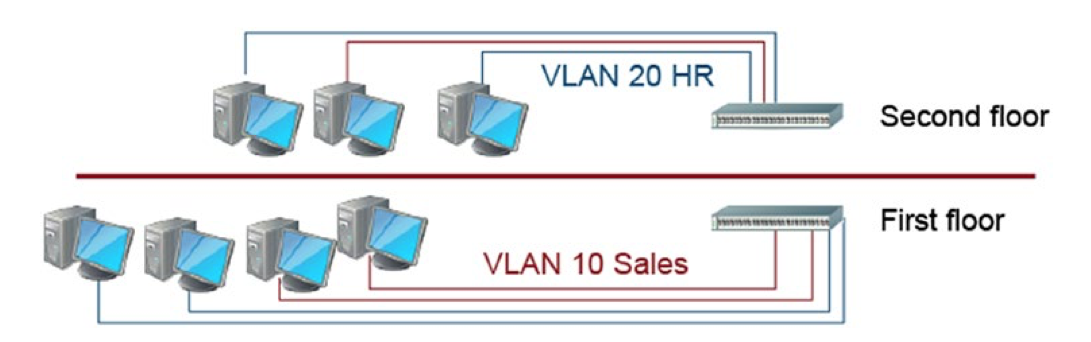
\includegraphics[width=\linewidth]{images/uploads/a_figure_08.png}
  \caption{Visuelle Darstellung der Aufteilung des Sales-Department, verbunden mittels VLAN. Quelle: \textcite{SheikhAhmedF2020CSCS}}
  \label{fig:VLAN}
\end{figure}
\bigbreak

VLANs können mittels \glqq{}Managed-Switches\grqq{} auf Basis von Port-Zuweisung oder \glqq{}Tagging\grqq{} realisiert werden. Bei Managed-Switches handelt es sich um Switches mit erweiterter Konfigurationsmöglichkeit wie etwa der gezielte Vergabe von IP-Adressen oder dem Filtering von MAC-Adressen \autocite{netgear}.
Beim portbasierten VLAN wird jedem VLAN ein spezifischer Port auf einem Switch zugewiesen, was in einem statischen VLAN resultiert. Im Gegensatz dazu wird beim tagged VLAN die Zuweisung dynamisch durchgeführt. Die Zuweisung zu einem VLAN erfolgt über eine Markierung (Tag) im Frame des Nachrichtenpakets. Auf Basis des Tags kann ein Switch erkennen in welchem Segment die Kommunikation stattfindet und das Paket entsprechend weiterleiten. Jedes VLAN besitzt seine eigene Broadcast-Domäne. \autocite{ionos_digitalguide}
\bigbreak
Die Verwendung von VLANs bringt unterschiedliche Vorteile mit sich \autocite{ionos_digitalguide}:
\begin{itemize}
    \item Flexibilität\\
    Änderungen an Teilnehmern des LANs können on-demand realisiert werden.
    \item Performance\\
    Durch die Reduzierung der Broadcast-Domäne wird unnötiger Traffic vermieden und die Bandbreite minimiert.
    \item Kostenersparnis\\
    Die Verwendung von VLANs ersetzt die Installation von parallelen physischen Netzen.
\end{itemize}
\bigbreak
Der größte Vorteil liegt allerdings am Sicherheitsgewinn, wenn große Netzwerke in kleine Gruppen segmentiert werden um damit den Zugang zu beschränken. Netzwerke können so auf Basis von VLANs nach belieben strukturiert und segmentiert werden. Nur Komponenten, die sich im selben VLAN befinden, können miteinander kommunizieren, ohne an Routern oder Firewalls vorbei zu müssen. Eine Kommunikation über Netzsegemente hinweg unterliegt der Kontrolle von Firewalls. \autocite{ionos_digitalguide}
\bigbreak
Firewalls kontrollieren eingehende und ausgehende Datenpakete und regulieren den Zugriff auf Komponenten innerhalb eines Netzwerksegments auf Basis von definierten Regeln. Es wird zwischen \glqq{}Packet-Filtering\grqq{}, \glqq{}Stateful Packet-Filtering\grqq{} und \glqq{}Deep Packet-Inspection\grqq{} unterschieden. In der einfachsten Ausführung überprüft eine Firewall ein- und ausgehende Datenpakete und entscheidet auf Basis von Regeln ob die Pakete die Firewall passieren dürfen. Stateful Packet-Filtering ist eine Weiterentwicklung dieser Überprüfung und bieten ein dynamisches Paketfiltering. So kann beispielsweise der gesamten Datenverkehr blockiert werden, wenn es sich nicht Responses zu ausgehenden Requests handelt. Deep Packet-Inspection bietet eine weitere Ausbaustufe und erlaubt der Firewall den Inhalt von Paketen zu analysieren und entsprechend auf diese Inhalte zu reagieren. \autocite{SheikhAhmedF2020CSCS}
\bigbreak
Mit Hilfe von VLANs und Firewalls lassen sich Unternehmens-Netzwerke in unterschiedliche Zonen unterteilen. Die Unterteilung kann auf Basis unterschiedlicher Ansätze erfolgen \autocite{the_bristol_group_deutschland_gmbh_2021}:
\begin{itemize}
    \item Trennung auf Basis pauschaler Sicherheitszonen
    \item Trennung nach Funktion oder Schutzbedarf
    \item Trennung nach Gerätetyp 
    \item Trennung nach Entwicklungs- und Produktionsumgebung
\end{itemize}
\bigbreak
Bei der Trennung auf Basis pauschaler Sicherheitszonen erfolgt eine erste grobe Segmentierung des Netzwerks. Mögliche Ausprägungen sind hierbei die Trennung in \glqq{}Vertrauenswürdige Zonen\grqq{}, \glqq{}Demilitarisierte Zonen (DMZ)\grqq{} und \glqq{}Management-Zonen\grqq{}. In vertrauenswürdigen Zonen befinden sich ausschließliche IT-Systeme mit bekannter Konfiguration und bekanntem Gesundheitsstatus. DMZ sind Zonen die den Austausch mit dem Interner in kontrolliert Art und Weise sicherstellen. IT-Komponenten innerhalb von DMZ exponieren sich im Internet. Auf diese Weise können Dienste wie E-Mail, Collaboration-Tools für Externe oder Webserver für Webseiten betrieben und aus dem Internet zugänglich gemacht werden. In der Regel werden DMZ zusätzlich über Perimeter-Firewalls, die den Zugriff auf nötige IP-Adressen und Ports beschränken, nach außen hin geschützt. Managed-Zonen sind Bereiche die ausschließlich Systeme zur Bereitstellung und Verwaltung der IT-Infrastruktur beheimaten. Ein Beispiel hierfür wäre ein zentraler Active-Directory Server \autocite{iainfoulds}. 
\bigbreak
Zusätzlich zu den pauschalen Sicherheitszonen können IT-Komponenten nach Geräteart oder auszuführender Funktion etabliert werden. So bietet sich eigene Segmente für Clients, Server oder etwa IP-Telefone an. Auf Basis der Trennung nach Funktion können zusätzliche Sicherheitsmechanismen, wie beispielsweise NAC etabliert werden. Mittels NAC kann einem Client zum Beispiel der Zugang zum Client-Segment verwehrt werden, wenn der Client nicht bestimmten Anforderungen entspricht. Mit Hilfe von NAC ist es somit möglich Clients mit einem veralteten Virenschutz automatisch in ein Quarantänenetz zu stellen. 
\bigbreak
NAC bietet des Weiteren folgende Funktionen \autocite{sandata_2022}:
\begin{itemize}
    \item Lokalisierung und Identifizierung neuer Geräte im Netzwerk
    \item Authentifizierung der Geräte 
    \item Zuweisung von Rollen und Berechtigungen
    \item Prüfung der Einhaltung festgelegter Sicherheitsrichtlinien
    \item Quarantäne-Zuweisung nicht-konformer Geräte
    \item Überwachung des Verhaltens der Endgeräte im Netzwerksegment
\end{itemize}
\bigbreak
Sowohl bei der Realisierung von Netzwerksegmentierung als auch bei Verwendung von NAC ist der Schutz von Vertraulichkeit und damit einhergehend die Absicherung der übertragenen Daten und des Netzwerkverkehrs unerlässlich. Diese Tatsache wird auch von Aufsichtsbehörden erkannt. Die EBA fordert, dass beim Austausch sensibler Zahlungsdaten über das Internet eine sichere Ende-zu-Ende-Verschlüsselung zwischen den kommunizierenden Parteien eingesetzt wird (Anforderungsmatrix Nummer 218). Zu diesem Zweck soll eine starke und weithin anerkannte Verschlüsselungstechnik verwendet werden. Auch die ESMA fordert, dass Daten bei der Übertragung verschlüsselt sein müssen (Anforderungsmatrix Nummer 415). Gerade für Banken ist die sichere Übertragung von Daten, nicht nur im Bereich des Online-Banking, unumgänglich um vertrauenswürdige Daten wie Passwörter oder Kreditkarten-Informationen zu schützen. Der vorherrschende Ansatz für die Verschlüsselung von Daten auf Transportebene ist die Verwendung von \glqq{}Transport Layer Security (TLS)\grqq{} beziehungsweise \glqq{}Secure Socket Layer (SSL)\grqq{}. \autocite{SchwenkJörg2020SuKi}

\subsubsection{Best-Practice-Ansatz: Verschlüsselung mittels SSL/TLS}
Kryptographie unterstützt bei der Wahrung der drei Sicherheitsziele \glqq{}Vertraulichkeit\grqq{}, \glqq{}Integrität\grqq{} und \glqq{}Authentizität\grqq{}. \textcite{SchwenkJörg2020SuKi} beschreibt die Erreichung der Sicherheitsziele durch Kryptografie wie folgt:
\begin{itemize}
    \item Vertraulichkeit\\
    Mit Hilfe von Verschlüsselungsalgorithmen ist es möglich, die Vertraulichkeit von Daten zu bewahren, damit nur die Besitzer eines bestimmten kryptographischen Schlüssels diese lesen können.
    \item Integrität\\
    Mit Hilfe eines gültigen \glqq{}Message Authentication Code\grqq{} (MAC) kann sichergestellt werden, dass Daten nicht verändert wurden \autocite{datatracker}. 
    \item Authentizität\\
    Die mit einer gültigen digitalen Signatur gesicherten Nachrichten können nur von der Person stammen, die den erforderlichen Schlüssel besitzt. Auf diesem Weg kann die Authentizität eines Teilnehmers gewährleistet werden. 
\end{itemize}
\bigbreak
Um die Sicherheitsziele zu gewährleisten besteht die Grundidee von SSL/TLS darin, einen verschlüsselten, transparenten und authentifizierten Kanal zur Verfügung zu stellen, über den Daten zwischen zwei Systemen zuverlässig übertragen werden können. 
\bigbreak
SSL in den Versionen 1.0 und 2.0 wurde 1994 von der Firma \glqq{}Netscape\footnote{https://isp.netscape.com}\grqq{}, zur Absicherung der Kommunikation über den Webbrowser \glqq{}Netscape Navigator\grqq{}, entwickelt. Aufgrund einiger Schwächen in Version 2.0 wurde die weitere Verwendung durch \glqq{}RFC 6176\grqq{} verboten \autocite{RFC6176}. SSL 3.0 wurde im Jahr 1996 veröffentlicht aufgrund einer Sicherheitslücke und des daraus resultierenden \glqq{}POODLE-Angriffs\grqq{} 2015 mittels \glqq{}RFC 7568\grqq{} verboten \autocite{RFC7568} \autocite{TA14-290A}. Im Jahr 1999 wurde SSL 3.1, als Upgrade auf SSL 3.0, unter der Bezeichnung TLS 1.0 veröffentlicht. TLS 1.0 wurde im Laufe der folgenden Jahre weiterentwickelt und neue Versionen im Jahr 2008 (TLS 1.2) und im Jahr 2018 (TLS 1.3) veröffentlicht. TLS 1.3 brachte große Änderungen, wie einen schnelleren Austausch von Nutzdaten und einem verkürzten Handshake mit sich. \autocite{SchwenkJörg2020SuKi}
\bigbreak
Folgende Funktionen werden von SSL/TLS angeboten \autocite{2022C}: 
\begin{itemize}
    \item Authentifikation von Server und Client auf Basis der Verwendung von Verschlüsselungsverfahren und elektronischen Zertifikaten.
    \item Vertrauliche Client-to-Server Datenübertragung unter Verwendung eines gemeinsamen Sitzungsschlüssel.
    \item Sicherstellung der Integrität der transportierten Daten unter Verwendung des HMAC-Verfahrens \autocite{HMAC}.
    \item Komprimierung von Daten 
\end{itemize}
\bigbreak
Eine SSL/TLS-Implementierung besteht auf Client- und Serverseite aus unterschiedlichen Komponenten \autocite{SchwenkJörg2020SuKi}:
\begin{itemize}
    \item Record-Layer\\
    Dieser bildet die grundlegende Komponente über die ein sicherer Kanal realisiert wird. Der Record-Layer empfängt einen Bytestrom, den er in \glqq{}Records\grqq{} aufteilt. Diese werden einzeln verschlüsselt, authentifiziert und mittels einer Sequenznummer miteinander verknüpft. 
    \item Handshake-Protokoll\\
    Mit Hilfe dieses Protokolls werden kryptographische Algorithmen und Schlüssel zwischen Client und Server ausgehandelt. Die Nachrichten des Handshake-Protokolls werden über den Record-Layer sowohl verschlüsselt als auch unverschlüsselt übertragen. 
    \item Change-Cipher\\
    \glqq{}Change-CipherSpec-Nachrichten\grqq{} signalisieren dem Record Layer den Wechsel vom unverschlüsselten in den verschlüsselten Modus. 
    \item Alert-Protokoll\\
    Über das Alert-Protokoll werden Fehlermeldungen zwischen Client und Server ausgetauscht. 
\end{itemize}
\bigbreak
Der TLS-Handshake, in dem der Schlüsselaustausch zwischen Client und Server stattfindet, bildet das Herzstück von TLS. Mit Hilfe des Schlüsselaustausches ist es den beteiligten IT-Systemen möglich verschlüsselt zu kommunizieren. Der TLS-Handshake baut nach \glqq{}RFC 5246\grqq{} auf der \glqq{}Diffie-Hellman-Schlüsselvereinbarung\grqq{} oder dem \glqq{}RSA-basierten Schlüsseltransport\grqq{} auf \autocite{RFC5246} \autocite{RFC5990}.
\bigbreak
Der Schlüsselaustausch wird durch die beiden Nachrichten \glqq{}Certificate\grqq{} und \glqq{}ClientKeyExchange\grqq{} im Zuge des TLS-Handshake realisiert. Hierbei sendet der Server seinen öffentlichen RSA-Schlüssel mit einem X.509-Zertifikat, in der \glqq{}Certificate\grqq{}-Nachricht an den Client \autocite{X509}. Der Client verschlüsselt daraufhin einen zufällig generierten 46-Byte-Wert zusammen mit der vom Client höchstmöglich unterstützten TLS-Version. Diese beiden Informationen bilden zusammen das \glqq{}Premaster Secret\grqq{}. Daraufhin verschlüsselt der Server das Premaster Secret mit dem öffentlichen Schlüssel des Servers und dem RSA-PKCS-Algorithmus und sendet den daraus resultierenden Chiffretext in der \glqq{}ClientKeyExchange\grqq{}-Nachricht zum Server \autocite{RSAPKCS}. Der Server wiederum kann den Chiffretext mit seinem privaten Schlüssel entschlüsseln \autocite{RFC3447}. Dieser Austausch wird von anderen beteiligten Nachrichten, wie in Abbildung \ref{fig:best-practice TLS-Handshake} ersichtlich, begleitet. \autocite{SchwenkJörg2020SuKi} 
\bigbreak
Der weitere Ablauf gestaltet sich wie folgt \autocite{SchwenkJörg2020SuKi}:
\begin{itemize}
    \item ClientHello\\
    Im Zuge der ClientHello-Nachricht werden die höchstmöglich unterstützte TLS-Version, eine Zufallszahl und eine Liste von möglichen kryptographischen Verfahren übergeben.
    \item ServerHello, Certificate, ServerHelloDone\\
    Nach Erhalt der ClientHello-Nachricht antwortet der Server mit einer Folge von Nachrichten (Entscheidung über gewähltes kryptographisches Verfahren, öffentlicher Schlüssel in Form eines X.509-Zertifikats) und schließt den Schritt mit ServerHelloDone ab. 
    \item ClientKeyExchange\\
    Der Client generiert einen zufällig Wert (PremasterSecret), verschlüsselt diesen mit dem öffentlichen Schlüssel des Servers und sendet diese Informationen an den Server.
    \item ChangeCipherSpec, Finished\\
    Der Server leitet aus dem PremasterSecret das MasterSecret ab, das als Ausgangspunkt für die Berechnung der kryptographischen Schlüssel dient. Nach Ableitung der Schlüssel kann der Client die vereinbarten Algorithmen aktivieren und den Handshake mittels ClientKeyExchange beenden. Der Server entschlüsselt die Nachricht ClientKeyExchange und leitet ebenfalls die Ableitung der Schlüssel durch. Im Anschluss daran aktiviert der Server die vereinbarten Algorithmen und beendet den Handshake mit der Nachricht ServerFinished.
\end{itemize}
\begin{figure}[H]
    \centering
  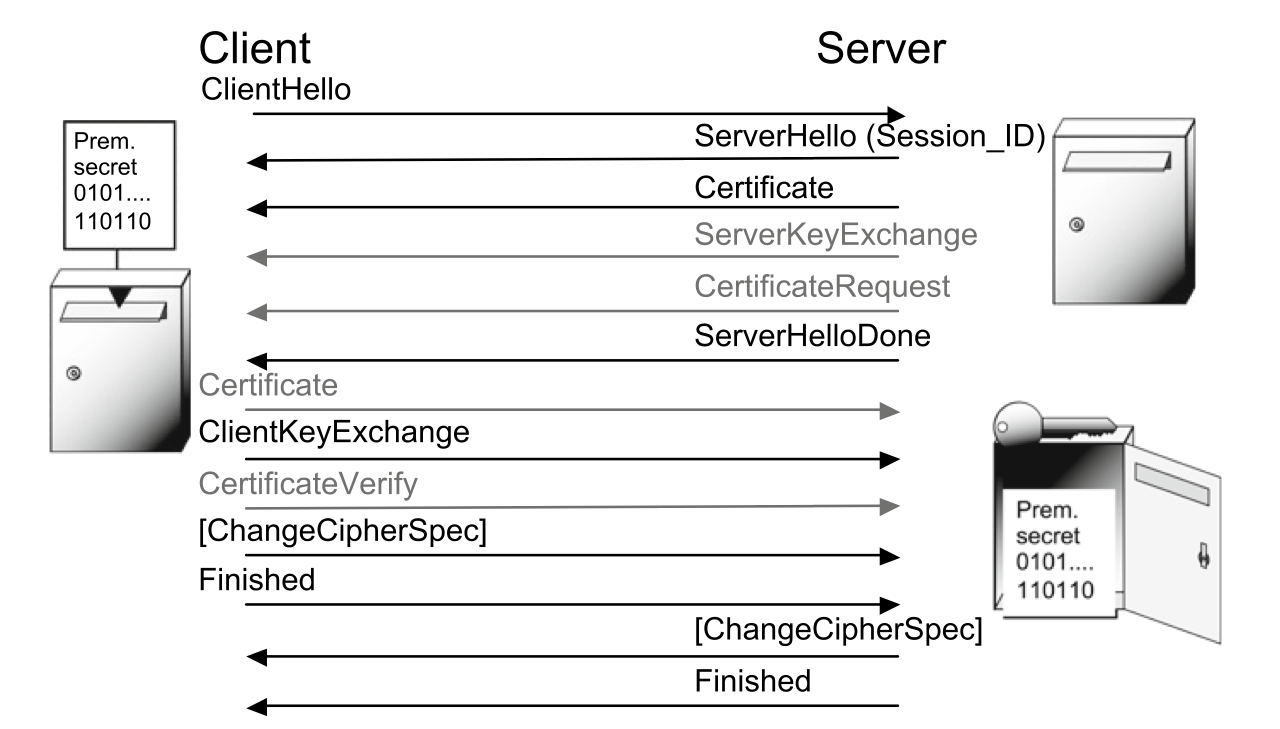
\includegraphics[scale=0.2]{images/uploads/a_figure_09.png}
  \caption{Schematische Darstellung eines TLS-Handshake mit RSA-basiertem Schlüsselaustausch. Quelle: \textcite{SchwenkJörg2020SuKi}}
  \label{fig:best-practice TLS-Handshake}
\end{figure}
\bigbreak
Nach erfolgreichem Handshake sind dem Server und dem Client untereinander jeweils folgende Informationen bekannt \autocite{SchwenkJörg2020SuKi}:
\begin{itemize}
    \item Die höchste vom Server und Client unterstützte TLS-Versionsnummer.
    \item Eine Ciphersuite mit einem Public-Key-Algorithmus zur Aushandlung des Premaster Secrets.
    \item Das definierte Master-Secret.
    \item Eine Session-ID.
    \item Der Verschlüsselungsschlüssel für den Datenverkehr zwischen Client und Server.
    \item Ein Schlüssel zur Generierung des MAC von Nachrichten für beide Übertragungsrichtungen.
\end{itemize}
\bigbreak
SSL/TLS wird von einer Vielzahl von Anwendungsprotokollen unterstützt und trägt somit zum Schutz der übertragenen Daten bei. Mit Hilfe von SSL/TLS kann beispielsweise eine verschlüsselte und integritätsgesicherte Verbindung für die Protokolle \glqq{}HTTP\grqq{}, \glqq{}SMTP\grqq{}, \glqq{}IMAP\grqq{}, \glqq{}FTP\grqq{} und \glqq{}Telnet\grqq{} realisiert und so den Anforderungen von Aufsichtsbehörden nachgekommen werden. \autocite{2022C}

\section{Cybersecurity-Management}
\label{Vulnerability-Management}
Die Gruppe \glqq{}Cyersecurity-Management\grqq{} vereint die Maßnahmen \glqq{}Security Incident Event Monitoring\grqq{} (SIEM), \glqq{}Log-Management\grqq{}, \glqq{}Vulnerability-Management\grqq{}, \\\glqq{}Penetration-Testing\grqq{} und \glqq{}Endpoint-Detection and Response\grqq{}. Die Gruppe beschäftigt sich mit der Erkennung von Angriffen auf IT-Systeme und dem aktiven Schutz dieser Komponenten.
\bigbreak
Der Bereich \glqq{}Cybersecurity\grqq{} deckt einen breiten Bereich an Bedrohungen und Maßnahmen ab, dem sich Banken in Österreich stellen müssen. Aufgrund der Relevanz stellen Aufsichtsbehörden unterschiedliche Anforderungen an die Cybersecurity von Banken. Die BaFin, die EBA und die FMA setzen voraus, dass Systeme für die automatische Erkennung von Anomalien und sicherheitsrelevanten Ereignissen eingeführt werden. Des Weiteren wird erwartet, dass sich Unternehmen ständig über laufende Bedrohungen und Schwachstellen des eigenen Informationsverbundes informieren, deren Relevanz prüfen und entsprechende Maßnahmen ergreifen. Aus diesem Grund haben Unternehmen ein Schwachstellenmanagement zur Erkennung, Bewertung und Behandlung von Schwachstellen zu implementieren (Anforderungsmatrix Nummer 19 und Nummer 31). Die FMA fordert des Weiteren, dass Unternehmen Maßnahmen zur Schwachstellenbeseitigung umsetzen. Unternehmen haben die Wirksamkeit der umgesetzten Maßnahmen laufend zu Überprüfung. Dies kann mittels Penetrationstests oder der Kontrolle von Logdaten durchgeführt werden (Anforderungsmatrix Nummer 265). 
\bigbreak
\subsubsection{Best-Practice-Ansatz: Aufbau Datenbasis - zentrales Logmanagement}
Ein erfolgreiches Cybersecurity-Management erfordert Kenntnisse über relevante Prozesse und Ereignisse innerhalb der IT-Struktur. Ein zur Verfügung stehendes Mittel, um Bedrohungen und Schwachstellen zu Identifizieren sind Logeinträge der im Netzwerk betriebenen IT-Systeme. Eine zentrale Forderung aus dem Bereich Cybersecurity der FMA an Unternehmen, ist die regelmäßige Erfassung und Auswertung von Logdaten der im Unternehmen verwendeten IT-Systeme (Anforderungsmatrix Nummer 261). Ein zentrales Logmanagement stellt geeignete Funktionen zur Übertragung, Speicherung, Analyse und Löschung von Logdaten zur Verfügung. 
\bigbreak
In folgendem Kapitel werden die grundlegenden Bestandteile eines zentralen Logmanagements erörtert und eine mögliche Implementierung, anhand des \glqq{}Elastic-Stacks\grqq{} (ELK-Stack), vorgestellt. \glqq{}ELK\grqq{} ist ein Akronym der im Framework enthaltenen Komponenten \glqq{}Elastic\grqq{}, \glqq{}Logstash\grqq{} und \glqq{}Kibana\grqq{} \autocite{ELK_Stack}.
\bigbreak

Für die Realisierung eines zentralen Logmanagements sind vorab unterschiedliche Überlegungen nötig: 
\begin{itemize}
    \item Welche Systeme sollen angebunden werden?\\
    Basierend auf den Betriebssystemen der jeweiligen Komponenten werden Programme zur Interpretation und Weiterleitung von Logeinträgen benötigt. 
    \item Welche Logdaten sollen übertragen werden?\\
    Werden sämtliche Logdaten eines Systems oder nur die Logdaten von bestimmten auf den Systemen betriebenen Applikationen benötigt?
    \item Wie lange sollen die Logdaten im zentralen Logmanagement gespeichert werden?\\
    Die Speicherung und Analyse von großen Mengen an Logdaten kann in einer erheblichen finanzielle Belastung resultieren.
\end{itemize}
\bigbreak
Auf Basis der genannten Überlegungen kommen unterschiedliche Komponenten für die Implementierung zum Einsatz. Am Beginn der Logmanagement-Pipeline stehen die einzelnen IT-Systeme, deren Logdaten gesammelt werden sollen. Abhängig vom Betriebssystem können die Logdaten beispielsweise mittels RSyslog\footnote{https://www.rsyslog.com}, für UNIX-Systeme, oder dem \glqq{}Windows-Event-Collector\grqq{} (WEC), für Windows Systeme, übertragen werden \autocite{WEC}. Die Logdaten werden in weiterer Folge an einen zentralen Logkollektor weitergeleitet. Für die Konstellation aus UNIX- und Windows-Systemen bietet sich Syslog-NG\footnote{https://www.syslog-ng.com} an, da dieser mit unterschiedlichen Betriebssystemen und Anwendungen kompatibel ist. Die Logdaten werden von Syslog-NG entgegengenommen und auf Basis der Quellen zwischengespeichert. Mittels einer Analysesoftware für Logdaten, wie beispielsweise \glqq{}Filebeat\grqq{}, Bestandteil des ELK-Stacks, werden die von Syslog-NG empfangenen Logeinträge in weiterer Folge ausgelesen und weiterbearbeitet. Im Anschluss daran werden die Logdaten mittels Logstash geparsed, gefiltert, normalisiert und an Elasticsearch weitergeleitet. Elasticsearch dient der Speicherung, Indexierung, Suche und Analyse von Logeinträgen. Mittels der Weboberfläche Kibana können die gespeicherten Logdaten grafisch dargestellt werden. Abbildung \ref{fig:best-practice logmanagement} zeigt die Schematische Darstellung einer mögliche Implementierung unter Verwendung des ELK-Stacks. 

\begin{figure}[H]
    \centering
  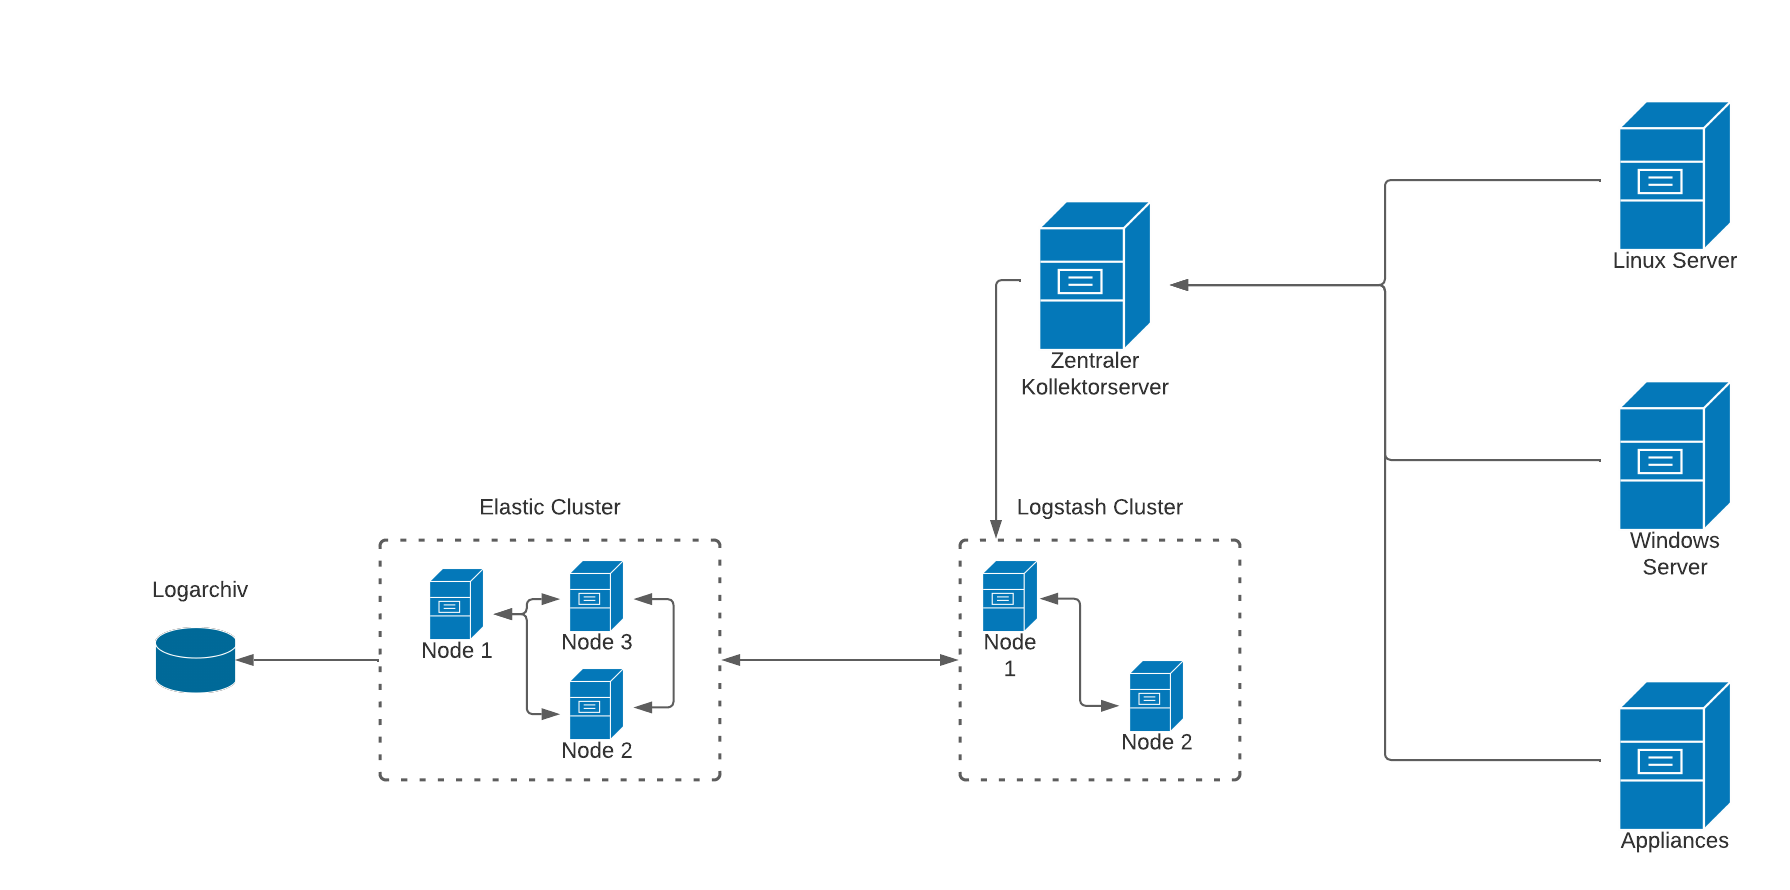
\includegraphics[scale=0.2]{images/uploads/a_figure_10.png}
  \caption{Schematische Darstellung eines zentralen Logmanagementsystems. Quelle: Eigene Darstellung, 2022}
  \label{fig:best-practice logmanagement}
\end{figure}
\bigbreak
Die Implementierung eines zentralen Logmanagementsystems kann folgende Vorteile mit sich bringen:
\begin{itemize}
    \item Erfüllung von Vorgaben der Aufsichtsbehörden.
    \item Etablierung eines zentralen Sammelpunktes für Logdaten.
    \item Möglichkeit zur zentralen Analyse sämtlicher Logdaten.
    \item Wahrung der Integrität der Logdaten (Logdaten auf den Systemen können von Angreifern gelöscht oder bearbeitet werden).
    \item Anbindung eines SIEM-Systems zur sicherheitstechnischen Analyse und Erkennung von Anomalien und Angriffsmustern.
\end{itemize}

\subsubsection{Best-Practice-Ansatz: Schwachstellen-Management}
Ein zentrales Logmanagement bietet die grundlegende Datenbasis für die Erkennung von Anomalien und Schwachstellen im IT-Netzwerk. Ein \glqq{}Security Information and Event Management\grqq{} System zentralisiert, korreliert und analysiert Daten im gesamten IT-Netzwerk in Echtzeit um etwaige Sicherheitsprobleme zu erkennen. Effizientes Log-Management ist für ein funktionierendes SIEM-System unerlässlich. Obwohl viele SIEM-Systeme aus diesem Grund auch die Funktionen eines zentralen Logmanagement-Systems bieten, wird diese Funktion aus Kostengründen häufig ausgelagert. Häufig werden SIEM-Systeme auf Basis der Menge an übertragenen Daten lizenziert und daher nur sicherheitsrelevante Logdaten vom zentralen Logmanagement in das SIEM-System importiert. Die Aufgabe eines SIEM-Systems ist es, schädliches Verhalten auf Basis vorliegender Logdaten zu identifizieren und Warnungen an die zuständigen Mitarbeiter zu senden. 
\bigbreak
Des Weiteren bieten führende SIEM-Systeme, wie etwa Splunk\footnote{https://www.splunk.com}, folgende Möglichkeiten \autocite{MehtaDeep2021SCSG}:
\begin{itemize}
    \item Überblick über relevante Events.
    \item Details zu relevanten Events.
    \item Möglichkeit zur Risikoanalyse von Systemen.
    \item Informationen über etwaige Bedrohungen.
    \item Informationen über beteiligte Prozesse bei einem Event.
    \item Definition von Usecases.
\end{itemize}
\bigbreak
SIEM-Systeme bieten die Möglichkeit eigene Usecases auf Basis von definierten Pattern zu erstellen. So besteht etwa die Möglichkeit der Implementierung einer \glqq{}Out-of-worktime Detection\grqq{} die alarmiert, falls Aktivitäten von privilegierten Accounts, außerhalb der üblichen Arbeitszeit, in den Logdaten gefunden werden. \autocite{MehtaDeep2021SCSG} 
\bigbreak
Die Implementierung eines SIEM-Systems setzt die von der EBA geforderten Maßnahmen an Banken zur Überwachung, Erkennung und Reaktion auf Sicherheitsvorfälle um. 
Häufig bieten SIEM-Systeme auch die Möglichkeit einer direkten Anbindung von Drittapplikationen, wie beispielsweise EDR-Systemen, an. EDR-Systeme bieten ähnlich wie SIEM-Systeme die Möglichkeit zur Überwachung auf Anomalien und sicherheitsrelevante Ereignisse in Echtzeit, basieren jedoch auf einem anderen Ansatz. Während ein SIEM-System auf Basis von erhaltenen Logdaten überwacht, wird bei der Überwachung mittels EDR meist ein Agent auf dem zu überwachenden IT-System installiert. 
\bigbreak
Der Agent bietet folgende Möglichkeiten:
\begin{itemize}
    \item Monitoring des zu überwachenden IT-Systems in Echtzeit.
    \item Sammeln relevanter Daten über das IT-System.
    \item Analyse der gesammelt Daten um Angriffsmuster oder Anomalien zu erkennen.
    \item Möglichkeit zur automatischen Quarantäne eines IT-Systems bei einem Sicherheits-Event.
    \item Möglichkeit zur forensischen Analyse im Zuge eines Sicherheits-Events.
\end{itemize}
\bigbreak
Ähnlich wie bei einem SIEM-System arbeiten EDR-Systeme auf Basis von Usecases. Ein bekannter Vertreter von EDR-Systemen ist Tanium.
\bigbreak
Eine weitere Möglichkeit zur Erkennung von Schwachstellen bietet das \glqq{}Vulnerability-Management\grqq{} (VuMa). Mit Hilfe von VuMa ist es möglich Sicherheitslücken in IT-Systemen und in den auf diesen Systemen laufenden Softwareprodukten zu erkennen, zu bewerten und diese zu melden. 
\bigbreak
Ein VuMa-Prozess kann in vier Schritte unterteilt werden \autocite{rapid7}:
\begin{enumerate}
    \item Schwachstellen erkennen
    \item Schwachstellen bewerten
    \item Schwachstellen behandeln
    \item Schwachstellen melden
\end{enumerate}
\bigbreak
Für die Erkennung von Schwachstellen auf IT-Systemen mittels VuMa, werden die IT-Systeme mit Hilfe eines Schwachstellenscanners überprüft. Hierfür wird das IT-Netzwerk nach zugänglichen Systemen untersucht und offene Ports oder Dienste auf den einzelnen IT-Systemen identifiziert. Es wird zwischen aktiven und passivem Scannen unterschieden. Beim aktiven Scannen interagiert der Scanner mit dem jeweiligen IT-System und bietet somit die Möglichkeit simulierte Angriffe auf das IT-System zu starten und Schwachstellen aktiv auszunutzen. Beim passiven Scannen werden detailliertere Systeminformationen gesammelt und die erhaltenen Systeminformationen in weiterer Folge mit bekannten Schwachstellen abgeglichen. Da sich das Scannen eines gesamten Netzwerkes zeitintensiv gestalten kann, können die erforderlichen Daten auch von EDR-Agents gesammelt und VuMa-Systemen zur Verfügung gestellt werden. \autocite{HaberMoreyJ2018AAV:}
\bigbreak
Werden auf einem IT-System Schwachstellen erkannt, müssen diese bewertet werden um das Risiko entsprechend behandeln zu können. VuMa-Systeme bieten meist unterschiedliche Risikobewertungen und Scores für gefundene Schwachstellen an. In der Praxis wird häufig nach dem \glqq{}Common Vulnerability Scoring System\grqq{} (CVSS) bewertet \autocite{CVSS}. Das tatsächliche Risiko einer Schwachstelle ist jedoch auch von weiteren Faktoren abhängig. 
\bigbreak
So sind folgende Punkte relevant \autocite{rapid7}:
\begin{itemize}
    \item Ist das betroffene IT-System aus dem Internet aus erreichbar?
    \item Welche Auswirkungen hat das Ausnützen der Schwachstelle auf den Betrieb?
    \item Handelt es sich um eine Schwachstelle oder ein False-Positive Ergebnis?
    \item Sind noch weitere Sicherheitsmaßnahmen vorhanden die ein Ausnützen der Schwachstelle verhindern könnten?
\end{itemize}
\bigbreak
Die Behandlung einer Schwachstelle erfolgt im besten Fall durch das Einspielen eines Patches mittels Patch-Management, wie in Kapitel \ref{Patch-Management} beschrieben. Existiert noch kein Patch oder ist das System bereits aus der Wartung, können unter Umständen mitigierende Maßnahmen zur Schadensbegrenzung gesetzt werden. Ziel ist es hierbei die Wahrscheinlichkeit eines Incidents, beziehungsweise möglichen resultierenden Auswirkungen zu reduzieren. Auch die Akzeptanz eine Schwachstelle und damit einhergehend dem ausbleibenden Setzen einer Maßnahme kann einer Behandlung entsprechen. Dies kann der Fall sein, wenn die Kosten der Behebung der Schwachstelle wesentlich höher sind als die Kosten, die einem Unternehmen entstehen wenn die Schwachstelle ausgenutzt wird. \autocite{rapid7}
\bigbreak
VuMa-Systeme bieten häufig die Möglichkeit automatisierte Scans durchzuführen und im Falle einer Schwachstelle zu alarmieren. Mittels eigens konfigurierbarer Dashboards kann der aktuelle Status der IT-Systeme auch grafisch dargestellt werden. 

\subsubsection{Prävention gegenüber Angriffen}
\label{ch:penetration-tests}
Präventive Maßnahmen zur Steigerung der Sicherheit von IT-Systemen schließen das Kapitel \ref{Vulnerability-Management} ab. 
Die FMA fordert, dass umgesetzte Maßnahmen zur Schwachstellenbeseitigung regelmäßig mittels Penetration-Tests überprüft werden. 
Obwohl sich die beiden Themen VuMa und Penetration-Testing in gewissen Bereichen überschneiden, bestehen grundlegende Unterschiede. Im Zuge des VuMa wird überprüft, ob eine Schwachstelle auf einem IT-System existiert oder nicht. Die Detektion kann auf Basis von einem fehlenden Update oder beispielsweise einem nicht gesetzten Windows Registry-Key geschehen. In den meisten Fällen kann im Zuge des VuMas nicht definiert werden ob andere mitigierende Maßnahmen implementiert sind, oder nicht. Im Gegensatz dazu wird bei einem Penetration-Test versucht die Sicherheitslücke aktiv auszunutzen um zu beweisen, dass eine Schwachstelle vorhanden ist und diese ausgenutzt werden kann. \autocite{HaberMoreyJ2018AAV:} 
\bigbreak
Es existieren unterschiedliche Ansätze und Ausprägungen von Penetration-Tests:
\begin{itemize}
    \item Black-Box Test\\
    Der Tester besitzt keinerlei Informationen über die zu testende IT-Infrastruktur. 
    \item White-Box Test\\
    Der Test besitzt Informationen über die IT-Infrastruktur, vorhandene Server, Betriebssysteme, offene Ports oder verwendete Dienste. Der Sinn eines White-Box Tests liegt in der gesteigerten Effizienz und wird verwendet, wenn ein bestimmtes System oder Verfahren getestet werden soll.
    \item Grey-Box Test\\
    Hierbei handelt es sich um eine Mischung aus Black-Box Test und White-Box Test. Dem Tester sind gewisse Informationen über das zu testende System, wie beispielsweise IP-Adressen Ranges, bekannt.
\end{itemize}
